%
%	SET ENVIROMENT FOR THESIS (PUCV) DOCUMENT
%

%\documentclass[letterpaper, twoside]{article}     	    %articulo tamaño carta
\documentclass[letterpaper, 11pt, twoside]{article}

% when two side is active, use the following lines
\raggedbottom
\usepackage[bottom]{footmisc}

\usepackage{booktabs} 								  	%Tablas bonitas de libro 
\usepackage[table,xcdraw]{xcolor} 					  	%tablas de latextable.com
\usepackage[english]{babel}				  				%Idioma						  
\usepackage[utf8]{inputenc} 						  		%Tildes y eñes
\usepackage{graphicx,epstopdf,pdfpages,float}		  	%Para poder insertar figuras, imagenes vectoriales, .pdf's y para fijar imagenes y tablas [H], resp.
\usepackage{latexsym,amsmath,amssymb,amsfonts,dsfont} 	%Caracteres propios de matematica, como el simbolo de los Reales
\usepackage{listings} 				                  	%Permite insertar codigos en C,MATLAB,ettc
\usepackage{color}									  	%Colour Fonts and other related features
\usepackage{multicol}[1999/05/25]					  	%Multiple Text Columns 	
\usepackage{subfigure}								  	%Subfigures
\usepackage{comment}

% User-defined commands (macros)
\providecommand{\abs}[1]{\lvert#1\rvert} 	  % Valor absoluto
\providecommand{\norm}[1]{\lVert#1\rVert}	  % Norma
\newcommand{\HRule}{\rule{\linewidth}{0.5mm}} % Linea Horizontal Bonita
\newcommand{\red}{\textcolor{red}}
\newcommand{\white}{\textcolor{white}}

% =============================================
% Customize section headers
\usepackage{titlesec}
\titlespacing*{\section}
{0pt}{12pt}{6pt}
%\titlespacing*{<command>}{<left>}{<before-sep>}{<after-sep>}
\newcommand{\ssection}[1]{\section[#1]{\fontsize{11}{12}\selectfont \centering #1}}
% to count sections witouth number
\makeatletter
% we use \prefix@<level> only if it is defined
\renewcommand{\@seccntformat}[1]{%
  \ifcsname prefix@#1\endcsname
    \csname prefix@#1\endcsname
  \else
    \csname the#1\endcsname\quad
  \fi}
% define \prefix@section
%\newcommand\prefix@section{Section \thesection: }
\newcommand\prefix@section{}
\makeatother

% =============================================
% Customize headers with fancy pagestyle
\usepackage{fancyhdr} \setlength{\headheight}{40pt}
%\rhead{} 
\lhead{\begin{figure}[H]

\includegraphics[height = 2 cm]{fig/logo_UCV}
\end{figure}}	% izquierda arriba  
%\chead{2}	% centro arriba
%\lfoot{3}	% izquierda abajo
%\cfoot{4}	% centro abajo
%\rfoot{5}	% derecha abajo
\renewcommand{\headrulewidth}{0pt} % grosor interfaz "header-documento"


% =============================================
% Other format options
% define vertical spacing between text lines
\usepackage{setspace}
% define indent size
\setlength\parindent{0cm}
% define space bewteen paragraphs
\setlength{\parskip}{6pt}
% Tipo de letra, margenes y estilo de pagina
%\renewcommand{\rmdefault}{phv} 		% Arial
%\renewcommand{\sfdefault}{phv} 		% Arial
%\usepackage[default]{gfsbodoni}		% Bodoni
\usepackage{mathptmx}					% Times New Roman
% Margenes: izquierda derecha arriba abajo
\usepackage{anysize}
\marginsize{4 cm}{2.5 cm}{0.65 cm}{2.5 cm}  	

\begin{document}

% =============================================
% TITLE PAGE
% Disable page-numbering for the titlepage
\pagenumbering{gobble}

\includepdf[pages=1]{./Portada/PORTADA.pdf}

%==============================================

% Re-enable page-numbering
\pagenumbering{arabic}
% Define vertical space for the rest of the document (equivalente a interlineado sencillo en Microsoft Word)
\spacing{1}
% Reset page counter in order to not consider the titlepage
\setcounter{page}{1}
% Set font size
\fontsize{11}{12}\selectfont

\tableofcontents
\newpage

% Consider abstract into table of contents
\addcontentsline{toc}{section}{RESUMEN} 
\addcontentsline{toc}{section}{ABSTRACT} 



\includepdf[pages=2]{./Abstract/Abstract.pdf}

\newpage

\section{INTRODUCTION}

In the human body under normal conditions, a self-regenerative process made by the organism  cells is done in order to repair cardiac cells regularly. Sometimes, the body overreact and as consequence produces an accumulation of connective tissue, consisting mostly collagen. This last can derive in fibrosis, which is in some conditions, a serious pathology because the normal conduction system of the heart may be altered, deriving in dyssynchrous heart failure and ventricular fibrillation (VF). Furthermore, ventricular fibrillation is the main cause of sudden cardiac arrhythmic death \cite{Myeburg_cardiac_sudden_death} in the United States, where heart failure accounts for over 280000 deaths each year \cite{American_heart_association_stathistics}. Therefore, the quantification of the relative amount of fibrotic tissue with respect to the healthy one may serve as an important biomarker for the assessment of cardiovascular risk.

In order to understand and, eventually, treat the fibrosis in a correct way, a more rigorous approach must to be taken. Mathematical electro-physiology offer us a complete model of the bio-electric cardiac sources and conducting media that allow to derive the electric potential over the heart tissue. Additionaly, the fibrotic tissue is a fibered material that introduces two scales of interest: the mesoscopic scale, i.e., at the level of myocite arrays and collagen incrustations ($\approx 0.1~[mm]$), and the macroscopic scale at the tissue level ($\approx 1 ~[cm]$).

To model the electric potential propagation over the tissue, we have to consider how the spatial distribution of the potential affect nearby cells, and how the cell itself respond to the stimulus. Typically, a reaction-diffusion model is used to achieve this. When ventricular fibrillation arises the normal sinus rhythm is disturbed when the same wavefronts continually re-excite the same tissue (re-entry); synchronous contraction of the ventricles is lost, circulation of the blood ceases and death occurs if normal sinus rhythm is not quickly restored. From the macroscopic point of view, this re-entry produced by the over stimulation of tissue generates electric potential spiral waves. Therefore, in order to diagnose a ventricular fibrillation by using only a computational simulation, the reaction-diffusion system has to reproduce well the spiral wave dynamics.

Some studies reveals that exist a close relation between the cardiac fibrosis spatial pattern and the velocity propagation of the potential. Indeed, the so-called \textsl{fibrosis architecture}, i.e., the spatial distribution of collagen fibers, affects more the wave propagation pattern than the intensity of fibrosis itself. Actual studies try to consider this by using different methods. For example, some studies emulate various kinds of fibrosis by randomly shut-down cells, assigning a different dispersion parameter for each one. Nevertheless, this does not emulates the meso-scale correctly. In order to do that this text proposes to explicitly model the myocites fibers and the connective tissue, and then reduce the computational cost of this by using some results of homogenization theory.


\section{GOAL AND OBJECTIVES}

The final goal is to model the electric potential propagation in a human fibrotic heart tissue. In order to do this, the following particular goals has to be achieved too:

\begin{itemize}
\item Model the electric propagation trough a reaction-diffusion system by using the so-called \textsl{Monodomain Equations}.
\item Compare different formulations for the reaction term in the Monodomain equations, such as Minimal and FitzHugh-Nagumo models.
\item Reduce the computational cost of the simulation using some results of the homogenization theory, preserving the meso-scale propierties with a effective macroscopic diffusion tensor.
\item Get homogenized electric potential fields over 2D domains that reproduce realistic conduction velocities.
\item Asses the error due to the introduction of effective diffusion tensor.
\item Simulate different spatial distributions of fibrosis, such as diffuse and stringy.
\end{itemize}


\ssection{BASIC CONCEPTS ON CARDIAC ANATOMY AND ELECTROPHYSIOLOGY} \label{Some_Basis_on_Anatomy_and_Electrophysiology}

The heart is a double pump consisting of four chambers, two atria in the upper part, separated by the inter-atrial septum and two ventricles in the lower part, separated by the inter-ventricular septum. See Figure \ref{corazon} for a hearth scheme and \cite{electrofis} for more details. 

\begin{figure}[!htbp] % esquema corazón
\centering
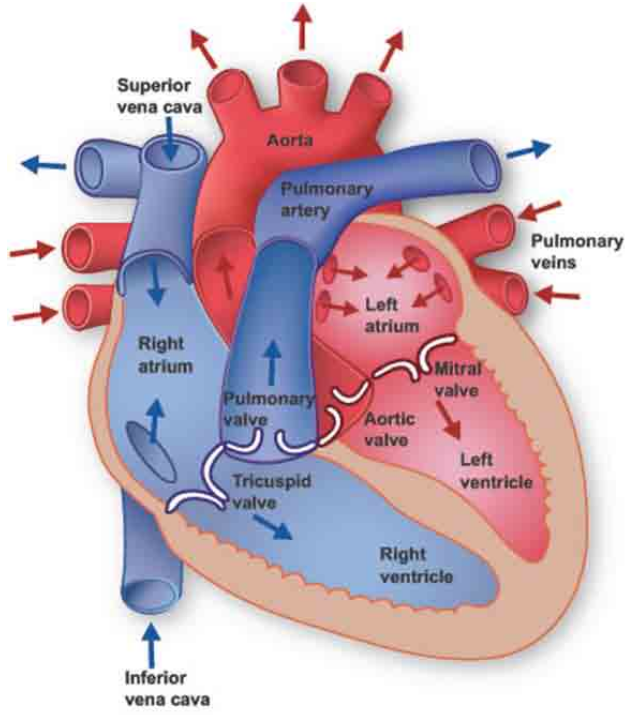
\includegraphics[height = 6 cm]{fig/fundamentals-corazon}
\caption{Schematic diagram of the heart anatomy.} \label{corazon}
\end{figure}

The electric potential wave genesis responsible of the cardiac muscle cells contraction occurs due to an autonomous depolarization in the sinoatrial node (SAN), located at the upper part of right atria. Then, the wave propagation is achieved because this depolarization changes the membrane potential of surrounding cardiac cells (due,  actually, to a cellular membrane ionic flow). The potential wavefronts travel first in the right atria, then into the left one. Next, the atrio-ventricular node (AVN) is reached, which conveniently has a high electric resistivity, in order to generate a control delay in the propagation, preventing any early ventricular stimulation. Finally, the Purkinge network (see Figure \ref{corazon_conduccion}) enable a fast potential propagation to ventricles chamber.

\begin{figure}[!htbp]% esquema conducción de corriente en el corazón
\centering
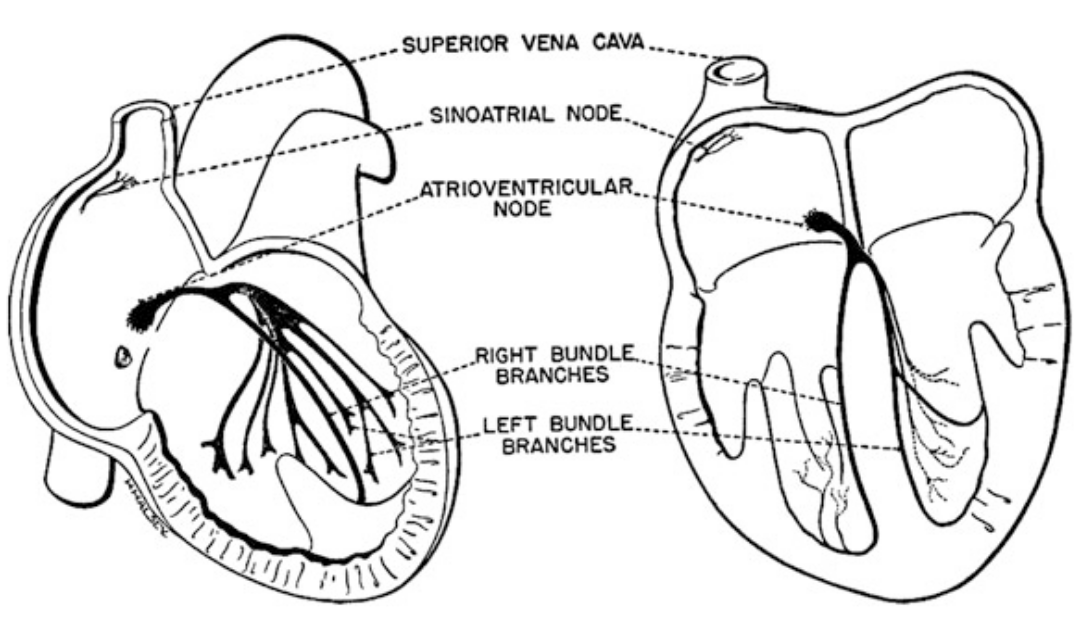
\includegraphics[height = 6 cm]{fig/fundamentals-sistema_de_conduccion}
\caption{Schematic diagram of the heart conduction system.} \label{corazon_conduccion}
\end{figure}

\subsection{Cardiac Tissue Organization} \label{Cardiac_Tissue_Organization}

The contract/relax macroscopic behavior of the heart is achieved due to collective cell activity. This cells, called myocites, works together joint by \textsl{gap junctions} which allows a quick electrical propagation in a particular direction, often called \textsl{the fiber direction}. Each one of this myocites has internal protein arrays called myofibrils, as can be seen in Figure \ref{fig:myocite}, which enables most part of the elastic properties of cardiac tissue.

Also, in the cardiac tissue exist another type of cells called \textsl{fibroblasts}, who are responsible of synthesize the extracellular matrix (ECM), an extensive and highly organized network of fibrous proteins, elastic and collagen (the main structural protein of the extra-cellular space in the human and other animals connective tissue). Specifically, the proportion of this last protein over the remain tissue can be used to measure fibrosis intensity.

\begin{figure}[!htbp]
	\centering
	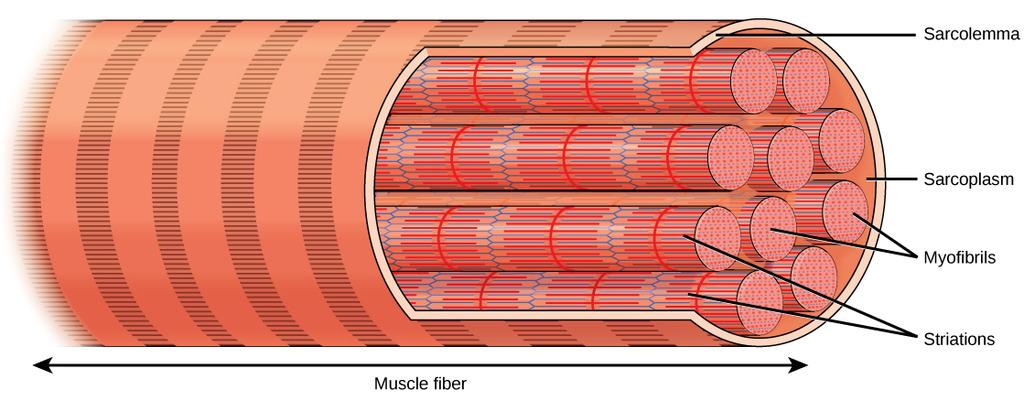
\includegraphics[height = 4 cm]{fig/fundamentals-myocites}
    \caption{Schematic view of a myocite.} 
    \label{fig:myocite}
\end{figure}

\begin{figure}[!htbp]
	\centering
    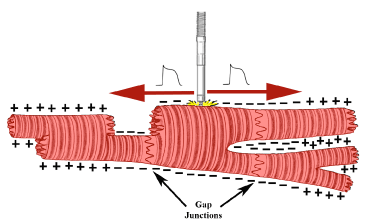
\includegraphics[height = 5 cm]{fig/fundamentals-gap_junctions} 
    \caption{Gap junctions: sarcoplasm electrical bypass of the myocites.}
    \label{fig:gap_junctions}
\end{figure}


Myocites and the ECM are arranged together within a complex three-dimensional spatial organization, with a fiber and laminar structure, like in Figure \ref{orientacionmiocitos}. This organization, as can be expected, affects the diffusion properties of the tissue, which is consequently highly anisotropic. This last usually is represented by a second-rank tensor, that can be written as a $3 \times 3$ matrix. The three orthogonal eigenvector of this tensor can be related directly to cardiac structure. In fact, the primary eigenvector (i.e. the eigenvector with largest eigenvalue) relays in the fiber long axis direction, the secondary eigenvector relays orthogonal to fiber long axis direction (cross-fiber direction), in the myolaminar plane, while the minor eigenvector, orthogonal to both fiber and cross-fiber directions, will be normal to the myolaminar plane.

\subsection{Action Potential} 

As established above, cardiac cells are excitable, some autonomously and some others after a proper electrical stimulus. The excitation of a cardiac cell causes a rapid variation of its potential difference across the cell membrane, the so-called \textsl{transmembrane potential}. There exist a minimum value of potential difference stimulus below the cell will react, a threshold, that if is reached, the cell membrane depolarizes and the trans-membrane potential changes from a resting negative value to a slightly positive one. This complete event is called an \textsl{action potential}, and phases can be identified, according to the activation of different membrane ionic channels. One action potential cycle can be seen in Figure \ref{action-potential}. 

\begin{figure}[!htbp]
\centering
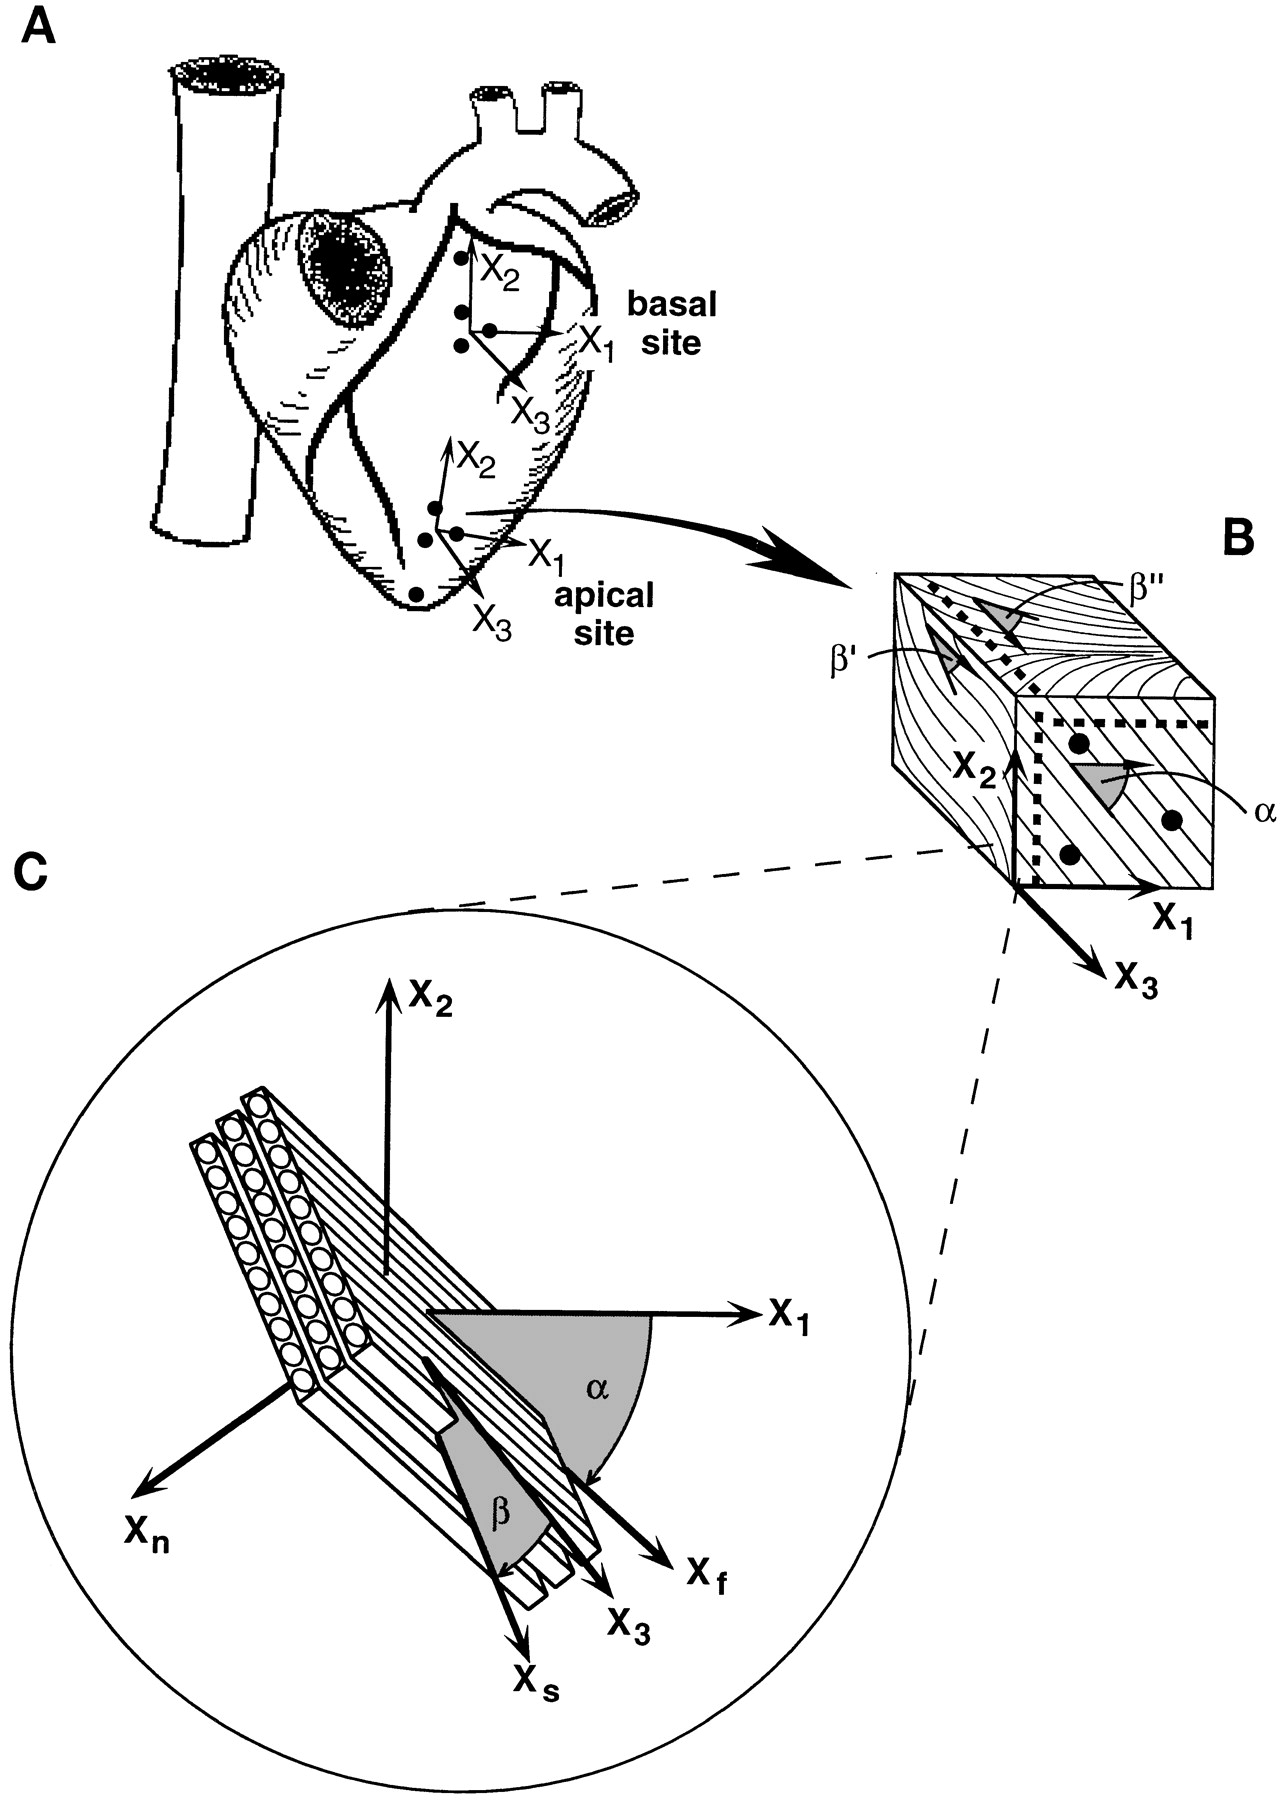
\includegraphics[scale=.14]{fig/fundamentals-direccionmiocitos}
\caption{Heart fiber orientation.} \label{orientacionmiocitos}
\end{figure}

The extracellular potential can be registered in a electrocardiogram (ECG), which can eventually lead us to diagnose some diseases as consequence of fibrosis, as the sinus bradycardia and tachycardia, arrhythmias, paroxysmal atrial tachycardia, etc.

\begin{figure}[!htbp]
\centering
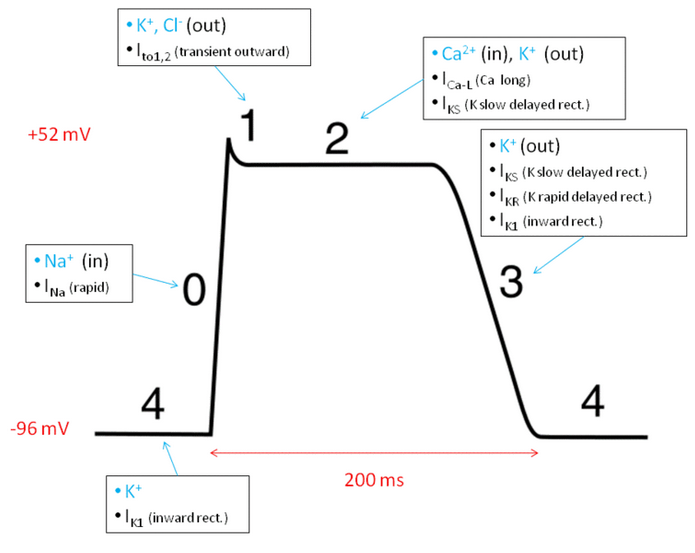
\includegraphics[height = 7 cm]{fig/fundamentals-action_potential}
\caption{Schematic plot of a cardiac action potential with its phases.} \label{action-potential}
\end{figure}

\subsection{Fibrosis} \label{Fibrosis}

Cardiac fibrosis is the excess of fibrous connective tissue, mostly collagen, as consequence of a self-regenerative process done by the fibroblasts. 

Different patterns of fibrosis has been observed accordingly to extra connective tissue percentage (density or intensity of fibrosis) and the dispersion of fibrotic areas in the tissue, i.e., the fibrosis architecture. Furthermore, according to this two statistical parameters, three types of fibrosis can be distinguished \cite{Kawara2001Circ}: \textsl{stringy}, \textsl{diffuse} and \textsl{patchy}. The stringy fibrosis architecture is characterized by homogeneously distributed collagen laminations with long and single strands. In patchy patterns arise long and compact groups of strands. Finally, diffuse fibrosis pattern is characterized with more or less homogeneously distributed small collagen short strands. The Figure \ref{fig:fibrosis_typology} shows the different types of fibrosis

The remarkable thing is that some studies \cite{Comtois2011IEEE} suggest that when a density threshold is reached, only spatial distribution of connective tissue affects the electric potential propagation velocity. In a recent research \cite{Kawara2001Circ}, the mean increase of the propagation delay (MID) was measured for failed human hearts with different fibrosis intensities. A result of this study can be seen in Figure \ref{fig:midvsdensity}, where the spatial distribution dependency of the parameter can be appreciated. Note that high values of MID are usually associated with patchy or stringy fibrosis. On the other hand, areas with diffuse fibrosis, low values of MID are found, even at high densities of fibrosis.

\begin{figure}[!htb]
\centering
\subfigure[Stringy Fibrosis.]{
    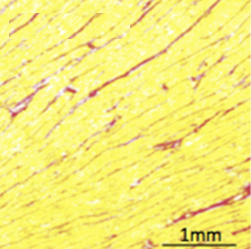
\includegraphics[height = 5 cm]{fig/fundamentals-fib-stringy}
    \label{fig:stringy}
}
\subfigure[Patchy Fibrosis. ]{
    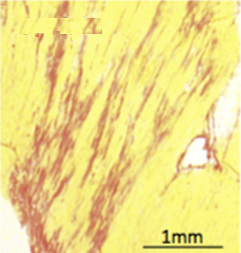
\includegraphics[height = 5 cm]{fig/fundamentals-fib-patchy} 
    \label{fig:patchy}
}
\subfigure[Diffuse Fibrosis. ]{
    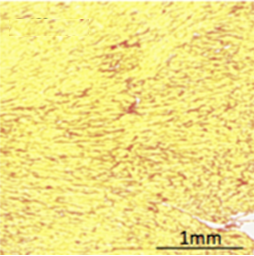
\includegraphics[height = 5 cm]{fig/fundamentals-fib-diffuse} 
    \label{fig:diffuse}
}
\caption{Different types of fibrosis.} \label{fig:fibrosis_typology}
\end{figure}



\begin{figure}[!htb]
	\centering
	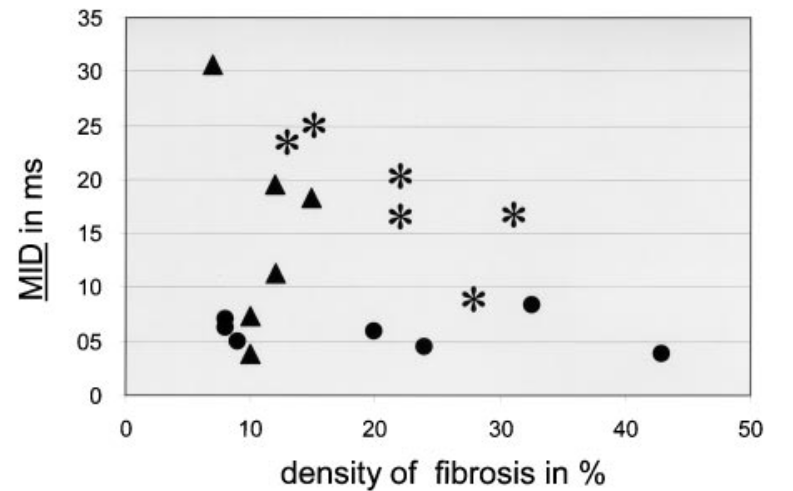
\includegraphics[height = 5 cm]{fig/fundamentals-fib-midvsdensity}
	\caption{Scatterplot of density of fibrosis and MID for different types of fibrosis (patchy, $*$; stringy, $\blacktriangle$; or diffuse, $\bullet$)}. \label{fig:midvsdensity}
\end{figure}


\section{MATHEMATICAL MODELS IN ELECTROPHYSIOLOGY}

Model the bio-electric cardiac source and the conducting media in order to derive the potential field is known as the \textsl{forward problem of electro-physiology}. There are different mathematical models that can achieve this goal, with more or less accuracy, as we will see in the followings paragraphs. 

\subsection{Cardiac Cells Arrangement Models}

Now we are going to present two mathematical models for the electric potential propagation over the cardiac tissue. For the mesoscopic scale is often used the so called bi-domain model, while for large problems at macroscopic scale the mono-domain model is usually used, mainly due to his computational low cost (in comparison with bi-domain model). The mathematical foundations, like the proof of existence and uniqueness of the solutions where performed by Colli Franzone and Savaré in \cite{colli_franzone}.

As general definitions, let us define $d$ as the dimension of the problem (usually 2 or 3), the domain $\Omega \subset \mathbb{R}^d$, and $\Gamma = \partial \Omega$ such that $\Gamma = \Gamma_D \cup \Gamma_N$ and $\Gamma_D \cap \Gamma_N = \emptyset$. Also, let us define the internal-variable vector that controls the cell membrane recovery (i.e. the action potential model) $\vec{r}: \Omega \times \mathbb{R}^+ \rightarrow \mathbb{R}^m$, where m is the number of parameters used to model the cellular membrane process.

\subsubsection{The Bi-Domain Model}

As far the author knows, the more detailed way to describe the potential propagation through the cardiac tissue is the bi-domain approach. This model establish an equation that describes the cardiac tissue considering the extra and intra cellular potentials separately. Furthermore, every cell membrane is considered as a capacitor, and separately, the resistivity of each ion channel in it (see Figure \ref{fig:bidomain_model}) is also considered. One way to express the anisotropic bi-domain model is trough the \textsl{PP-formulation}, that is enunciated in the next paragraph.

\begin{figure}[H]
\centering
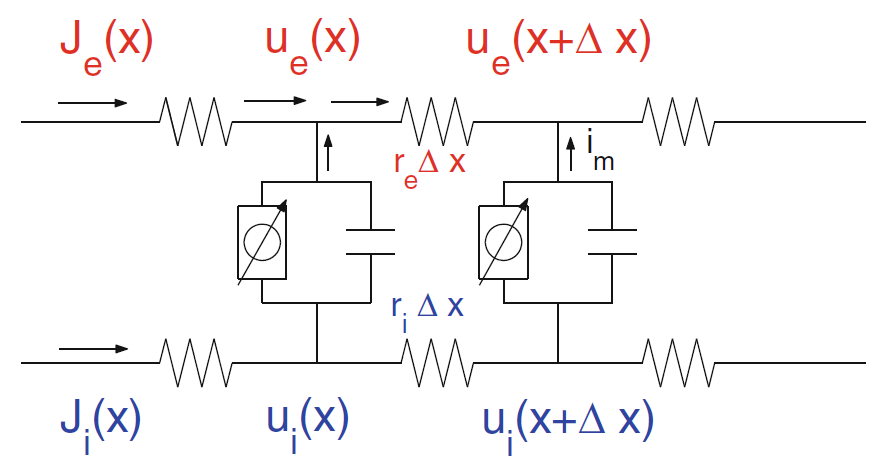
\includegraphics[scale=.35]{fig/cable_model}
\caption{Bi-domain model squeme.} \label{fig:bidomain_model}
\end{figure}

\textbf{PP-formulation:} Let us define the intern and extra cellular conductive tensors $D_i$ and $D_e$, respectively. Given the applied intra and extracellular currents per units volume $I_{i,e}^s: \Omega \times (0,T) \rightarrow \mathbb{R}$, and initial conditions $v_0 : \Omega \rightarrow \mathbb{R}$, $w_0: \Omega \rightarrow \mathbb{R}^k$, $z_0: \Omega \rightarrow (0, +\infty)^m$, find the intra and extracellular potentials $u_{i,e}:\Omega \times (0,T) \rightarrow \mathbb{R}^k$ and the ionic concentrations variables $\vec{r}: \Omega \times (0,T) \rightarrow \mathbb{R}^m$ such that:

\begin{equation}
\arraycolsep=1.4pt\def\arraystretch{2.2}
\begin{array}{rlr}
c_m \dfrac{\partial v}{\partial t} - div(D_i \nabla u_i) + I_{ion}(u_{i,e}, \vec{r}) &= I_{i}^s & \text{ in } \Omega \times (0,T) \\
-c_m \dfrac{\partial v}{\partial t } - div(D_e \nabla u_e) - I_{ion}(u_{i,e}, \vec{r}) &= I_e^s & \text{ in }\Omega \times (0,T) \\
\end{array}
\label{eq:BDM}
\end{equation}

The reaction term $I_{ion}$ and the ODE system for the gating variables are given by the cellular membrane electrical activity model. 

\subsubsection{The Mono Domain Model}

The bi-domain model is highly computational expensive because of the involvement of different space and time scales. Indeed, a complete heartbeat can last nearly 1 second, while the time constants of the rapid kinetics involved ranges from 0.1 to 500 ms. For the space scale, are involved portions of cardiac tissue of the order of centimeters, while the electric potential propagates trough layers of the order of a tenth of a millimeter.

Since the above, usually the \textsl{mono-domain model} equations are solved for large domains, which are a simplification of the bi-domain model. Let us define the following:

\begin{itemize}
\item The scaled transmembrane potential $\phi: \Omega \times \mathbb{R^+}$.
\item The conductivity tensor $D \in \mathbb{R}^{d \times d}$.
\end{itemize}

The mono-domain model can be written as follows:

\begin{equation}
\arraycolsep=1.4pt\def\arraystretch{2.2}
\begin{array}{rl}
\dfrac{\partial \phi}{ \partial t} - div(D \nabla \phi) &= I_{ion} (\phi, \vec{r}) \\
\end{array}
\label{eq:MDE}
\end{equation}

The interpretation of $I_{ion} (\phi, \vec{r})$ is subjected to the choice of the cell electrical activity model. Also note that the Fick's first diffusion law has been adopted.

Finally, in order to reproduce the cardiac tissue properties from a macroscopic point of view, the diffusion tensor is often taken as follows:

\begin{equation}
D = d_1 \hat{f} \otimes \hat{f} + d_2 \hat{c} \otimes \hat{c} \label{eq:macroscopic_diff_tensor}
\end{equation}

where $d_1$ and $d_2$ are the diffusivity for principal and transverse fiber directions, respectively, which are described by unit vectors $\hat{f}$ and $\hat{c}$. The tissue anisotropy will be considered by setting $d_1 = \gamma                                    
d_2$, with $\gamma > 1$. 

\subsection{Cellular Membrane Electrical Activity Models}

\subsubsection{FitzHugh-Nagumo Model}

To describe the source $I_{ion}$, the FitzHugh-Nagumo (FHN) reduced ionic model can be used, which can be written as follows:

\begin{align}
I_{ion}(\phi, w) &= c_1 \phi (\phi - \alpha)(1 - \phi) - c_2 w \\
\dfrac{\partial w}{\partial t} &= c_2 (\phi - wd) \nonumber
\end{align}


where $c_1$, $c_2$ and $d$ are real positive numbers, representing the excitation rate, the excitation decay and the recovery decay of the cell, respectively. Note that we are using the transmembrane potential $\phi$ to write the model, but eventually the FHN equations can be plugged in the bi-domain equations too. In this case, only one recovery variable models the whole membrane electrical activity, therefore the recovery variable vector has only one component, i.e., $\vec{r} = w$.


\subsubsection{Minimal Ventricular Model} 

Other accepted model for the membrane electrical activity is the so called \textsl{Minimal Model} proposed by Bueno-Orovio \cite{BUENO_OROVIO_MINIMAL}. This model takes in account three gating variables, let say $\vec{r} = (r,w,s)$, and can be written as follows:

\begin{equation}
\arraycolsep=1.4pt\def\arraystretch{1.5}
\begin{array}{lr}
I_{ion}(\phi, r, w, s) = - (J_{fi} + J_{so} + J_{si}) \\ 
\partial_t r = (1 - H(\phi - \theta_v))(r_\infty - r)/\tau_{v}^- - H(\phi - \theta_v)r/\tau_v^+ \\
\partial_t w = (1 - H(\phi - \theta_w))(w_\infty - w)/\tau_{w}^- - H(\phi - \theta_w)w/\tau_w^+ \\
\partial_t s = ((1 + tanh(k_s(\phi - \phi_s)))/2 - s)/\tau_s
\end{array} \label{eq:mde_min}
\end{equation}

where $H:\mathbb{R} \rightarrow \mathbb{R}$ is the heaviside function, defined by:

\begin{equation}
\arraycolsep=1.4pt\def\arraystretch{1.5}
H(x) = 
\left\lbrace
\begin{array}{lr}
1 & if~~x > 0 \\
0 & if~~x \leq 0
\end{array} 
\right. \label{eq:HS}
\end{equation}

and where,

\begin{equation}
\arraycolsep=1.4pt\def\arraystretch{1.5}
\begin{array}{lr}
J_{fi} = -r H(\phi - \theta_r)(\phi - \theta_r)(\phi_u - \phi)/ \tau_{fi} \\
J_{so} = (\phi - \phi_0)(1 - H(\phi - \theta_w))/\tau_o + H(\phi - \theta_w)/\tau_{so} \\
J_{si} = -H(\phi - \theta_w)ws/\tau_{si} 
\end{array} \label{eq:mde_currents}
\end{equation}

are the trans-membrane currents considered (fast inward, slow inward and slow outward). It has been shown that this variables retain enough information about cardiac excitation to reproduce exact AP morphologies. This last plus the three gating variables allows to model an action potential that can reproduce arbitrary action potential duration (APD) and conduction velocity (CV) restitution curves.

Also, the Bueno-Orovio model needs the following definitions:

\begin{equation}
\arraycolsep=1.4pt\def\arraystretch{1.5}
\begin{array}{lr}
\tau_r^- = (1 - H(\phi - \theta_r^-))\tau_{r1}^- + H(\phi - \theta_r^-)\tau_{r2}^- \\
\tau_w^- = \tau_{w1}^- + (\tau_{w2}^- - \tau_{w1}^-)(1 + tanh(k_w^- (\phi- \phi_w^-)))/2 \\
\tau_{so} = \tau_{so1} + (\tau_{so2} - \tau_{so1})(1 + tanh(k_{so}(\phi - \phi_{so})))/2 \\
\tau_s = (1 - H(\phi - \theta_w))\tau_{s1} + H(\phi - \theta_w)\tau_{s2} \\
\tau_0 = (1 - H(\phi - \theta_i)) \tau_{o1} + H(\phi - \theta_o) \tau_{o2} \\
\end{array} \label{eq:mde_parameters}
\end{equation}

and,

\begin{equation}
r_{\infty} = \left\lbrace \begin{array}{cr}
1 & \phi < \theta_r^- \\
0 & \phi \geqslant \theta_r^-
\end{array} \right.
~~~~~~~~w_{\infty} = (1 - H(\phi - \theta_o))(1 - \phi/\tau_{w\infty}) + H(\phi - \theta_o)w_{\infty}^*
\end{equation}


For remain parameters see table \ref{tab:parametros_minimal}, where four sets of values are shown for different layers of the  hearth's wall, i.e., for epicardium (EPI), mid-myocardial (MID), epicardial (EPI) and for the atrial tissue. Parameters were taken from Bueno-Orovio results in \cite{BUENO_OROVIO_MINIMAL} and \cite{MINIMAL_ATRIAL}. 


% Please add the following required packages to your document preamble:
% \usepackage{booktabs}
\begin{table}[H]
	\centering
	\caption{Four different set of parameters for cell Minimal Model.}
	\label{tab:parametros_minimal}
	\begin{tabular}{@{}cccccc@{}}
		\toprule
		id & Parameter     & EPI    & ENDO   & MID    & ATRIAL \\ \midrule
		1  & $\phi_0$      & 0      &        & 0      & 0      \\
		2  & $\phi_u$      & 1.55   & 1.56   & 1.61   & 1.02   \\
		3  & $\theta_r$    & 0.3    & 0.3    & 0.3    & 0.302  \\
		4  & $\theta_w$    & 0.13   & 0.13   & 0.13   & 0.33   \\
		5  & $\theta_r^-$  & 0.006  & 0.2    & 0.1    & 0.172  \\
		6  & $\theta_0$    & 0.006  & 0.006  & 0.005  & 0.06   \\
		7  & $\tau_{r1}^-$ & 60     & 75     & 80     & 65.6   \\
		8  & $\tau_{r2}^-$ & 1150   & 10     & 1.4506 & 1150   \\
		9  & $\tau_r^+$    & 1.4506 & 1.4506 & 1.4506 & 0.95   \\
		10 & $\tau_{w1}^-$ & 60     & 6      & 70     & 170.8  \\
		11 & $\tau_{w2}^-$ & 15     & 140    & 8      & 112.4  \\
		12 & $k_w^-$       & 65     & 200    & 200    & 135    \\
		13 & $\phi_w^-$    & 0.03   & 0.016  & 0.016  & 0.744  \\
		14 & $\tau_w^+$    & 200    & 280    & 280    & 217    \\
		15 & $\tau_{fi}$   & 0.11   & 0.1    & 0.078  & 0.0678 \\ 
		16 & $\tau_{o1}$       & 400     & 470    & 410 & 100   \\
		17 & $\tau_{o2}$       & 6       & 6      & 7 & 64.87     \\
		18 & $\tau_{so1}$      & 30.0181 & 40     & 91 & 53.54    \\
		19 & $\tau_{so2}$      & 0.9957  & 1.2    & 0.8 & 8.03   \\
		20 & $k_{so}$          & 2.0458  & 2      & 2.1 & 1.748   \\
		21 & $\phi_{so}$       & 0.65    & 0.65   & 0.6 & 0.644   \\
		22 & $\tau_{s1}$       & 2.7342  & 2.7342 & 2.7342 & 5.406 \\
		23 & $\tau_{s2}$       & 16      & 2      & 4 & 52.91     \\
		24 & $k_s$             & 2.0994  & 2.0994 & 2.0994 & 1.008 \\
		25 & $\phi_s$          & 0.9087  & 0.9087 & 0.9087 & 0.814 \\
		26 & $\tau_{si}$       & 1.8875  & 1.9013 & 3.3849 & 6.978 \\
		27 & $\tau_{w \infty}$ & 0.07    & 0.0273 & 0.01 & 4.97  \\
		28 & $w_{\infty}$         & 0.94    & 0.78   & 0.5 & 1   \\ \hline
\end{tabular}
\end{table}


\subsection{Homogenization}

Due to the multiscale nature of the problem, the application of some results from the Homogenization theory \cite{homogenization} can improve the computational performance in coarse meshes still preserving the influence of the mesoscopic configuration into the macroscopic scale.

\subsubsection{Homogenization Theorem for Diffusion Equations}

\subsubsection*{Rank 1 Laminations}

First, we gonna verify a homogenization theorem for a static diffusion problem over a domain with two materials, where one of them is laminated over the other, in order to eventually expand the theorem beyond his boundaries (where has no formal proof, as the case with a reaction term). So, let us consider two materials, $d_1$ and $d_2$, with $D_1$ and $D_2$ constant diffusion tensors, respectively. Also, let us define $\theta \in \mathbb{R}$ the proportion of the material $D_1$ over the rest of the domain and $e_1 \in \mathbb{R}^d$ the lamination direction (see Figure \ref{fig:lamination_fig}), which is orthogonal to the fiber direction.

Homogenization theory has been a very succesfull mathematical theory dealing with linear difussion equations (and many other systems). However, up to the knowledge of the authors, there are no newer results to be directly applied to the nonlinear and coupled system described, e.g., in \ref{eq:mde_min}. Nevertheless, we propose to apply, as a linear approximation to the full nonlinear homogenization system, the following surrogate model for the effective diffusion tensor:

\begin{equation}
D^{eff} = \theta D_1 + (1 - \theta) D_2 - \frac{\theta (1 - \theta)(D_1 - D_2)e_1 \otimes (D_1 - D_2)^T e_1}{(1 - \theta)D_1 e_1 \cdot e_1 + \theta D_2 e_1 \cdot e_1 } \label{eq:homogenization_rank1}
\end{equation}

This formula was first obtained by Murat and Tartar in 1978 and applies to linear difussion. We claim that nonlinear effects, eventhough they were not originally considered within these calculations, should not significantly affect the full effective tensor (if exists) by assuming that $I_{ion}$ is bounded in proper functional settings and since the nonlinearities studied here do not include derivatives. Once accepted this surrogate model (indistinctly called homogenized model), one can easily go further by applying sequential laminations as in the sequel.

\begin{figure}[!htbp]
\centering
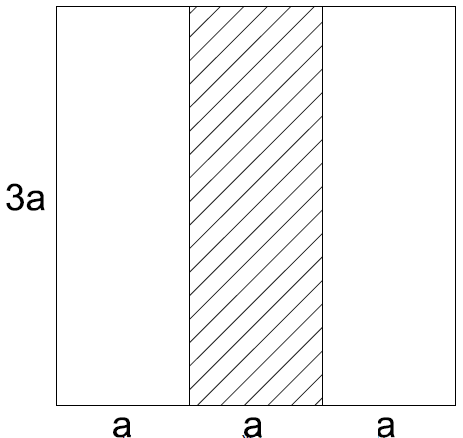
\includegraphics[height = 5 cm]{fig/theorem_verification_r1-ejemplo_laminaciones} 
\caption{Example of a domain with two materials. In this case, the proportion is $\theta = 1/3$ and lamination direction $e_1 = (1,0,0)$.} \label{fig:lamination_fig}
\end{figure}

\subsubsection*{Rank 2 Laminations}

Since in the heart, a more realistic configuration must also consider that healthy cells are slightly separated by collagen, the lamination formula can be repeated once again to reproduce such characteristical pattern (see Figure \ref{fig:geometry_convention}):

\begin{figure}[!htbp]
\centering
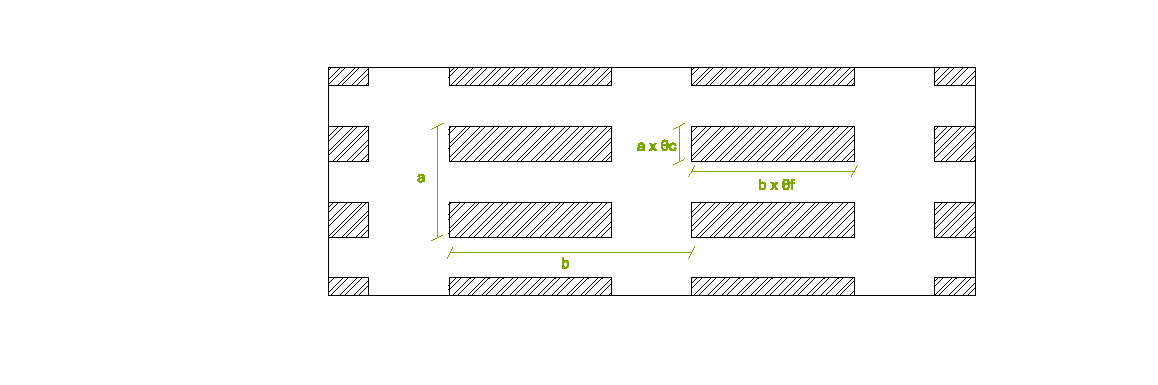
\includegraphics[height = 5 cm]{fig/theorem_verification_r2-geometry_convention} 
\caption{Geometric configuration of the mesoscopic scale of the heart tissue.} \label{fig:geometry_convention}
\end{figure}

Let us consider two laminations directions defined by the local basis $e_1$ and $e_2$, and a collagen diffusion tensor defined as $D_{col} = d_{col} I_{2 \times 2}$, where $d_{col}$ is the collagen diffusivity. Also, let us consider a domain with only collagen within, and the laminations of healthy tissue described by $\hat{f}$ with direction $e_1$. The effective tensor for this configuration will be, according with \ref{eq:homogenization_rank1}:

\begin{equation}
D_{eff}'=
(1 - \theta_c)D_h + \theta_c D_{col} - \frac{\theta_c (1 - \theta_c)(D_{col} - D_{h})e_1 \otimes (D_{col} - D_{h})^T e_1}{(1 - \theta_c)D_{col} e_1 \cdot e_1 + \theta_c D_{h} e_1 \cdot e_1 }
\end{equation}

Having this, we can proceed to laminate with healthy tissue in the cross direction, considerering now an array of laminations described by $\hat{c}$ (with lamination direction $e_2$) inside a domain with a diffusion tensor $D_{eff}'$. So that, if $D_{eff}$ is the effective diffusion tensor for the domain with the two array of laminations, we can write:

\begin{equation}
D_{eff} = 
(1 - \theta_f)D_h + \theta_f D_{eff}' - \frac{\theta_f (1 - \theta_f)(D_{eff}' - D_h)e_2 \otimes (D_{eff}' - D_h)^T e_2}{(1 - \theta_f)D_{eff}' e_2 \cdot e_2 + \theta_f D_h e_2 \cdot e_2 }
\end{equation}

\section{NUMERICAL EXPERIMENTS}

\subsection{Experiment \# 0: Linear Diffusion}

In this section the enunciated homogenization theorem will be numerically validated first in a linear setting (only diffusion). To do this, we can write the problem \eqref{eq:MDE} neglecting the reaction term and using the following variational approach: find  $\phi^{n+1}$ such that:

\begin{equation}
\int_{\Omega} \phi^{n+1} ~v ~d \Omega+ \Delta t \int_{\Omega} (D \nabla \phi^{n+1}) \cdot \nabla v ~ d \Omega  = \int_{\Omega} \phi^{n} v ~ d \Omega + \Delta t  \int_{\Gamma_N} g v ~ ds  \label{eq:diff_weak_form}
\end{equation}

where $v \in V$, $V = \{ v \in H^1(\Omega)\}$. The Backward Euler method was used to discretize the temporal variable, i.e., $\dot{\phi} = (\phi^{n+1} - \phi^{n})/\Delta t$, where $\Delta t$ is the time step and $\phi^{n+1}$ is the resolved potential field at the previous time-step.

Let us start by setting a two-dimensional problem ($d = 2$) considering $\Omega = [0,25 \text{mm}]\times[0, 25 \text{mm}]$. The diffusion tensor will be taken as \eqref{eq:macroscopic_diff_tensor}, using the parameters of table \ref{tab:parameters_tensor}:

\begin{table}[!htbp]
	\centering
	\caption{common parameters for numerical experiments.}
	\label{tab:parameters_tensor}
	\begin{tabular}{@{}ccc@{}}
		\toprule
		Paramter & Meaning                & Value        \\ \midrule
		$d_1$    & main fiber diffusivity & 0.1  $[mm/s]$ \\
		$\gamma$ & defined below   & 4            \\
		$\beta$ & defined below           & 5            \\
		$\hat{f}$ & main fiber direction  & $(1,~0)$           \\
		$\hat{c}$ & cross fiber direction & $(0,~1)$            \\ 
		$I_{dur}$ & stimulus duration    & 3 $[ms]$           \\
		$a$ & radius of the myocites array with collagen & 0.1  [mm]       \\ 
		$b$ &\begin{tabular}[c]{@{}c@{}}distance between the start of two contiguous collagen\\ inclusions (in direction $e_2$)\end{tabular}    & 1 [mm]  
		\\ \bottomrule
	\end{tabular}
\end{table}


where $\beta$ is defined by $d_{col} = 10^{-\beta} \times d_1$ and $d_2 = d_1/\gamma$. So, the collagen diffusion tensor is taken as $D_{col} = d_{col} \times \mathbb{I}_2$. The boundary condition is taken as a constant Neumann stimulus at the left edge of intensity $I_{est} = 50$ and duration $I_{dur}$. In the other boundaries just zero Neumann boundary conditions are asumed. Also, zero initial conditions are assumed over all the domain.

The geometry for simulation is shown in figure \ref{fig:geometry}. The materials proportions were chosen as $\theta_c = 0.4$ and $\theta_f = 0.5$ (highly fibrotic tissue). The time step is $1~[ms]$.

\begin{figure}[!htbp]
	\centering
	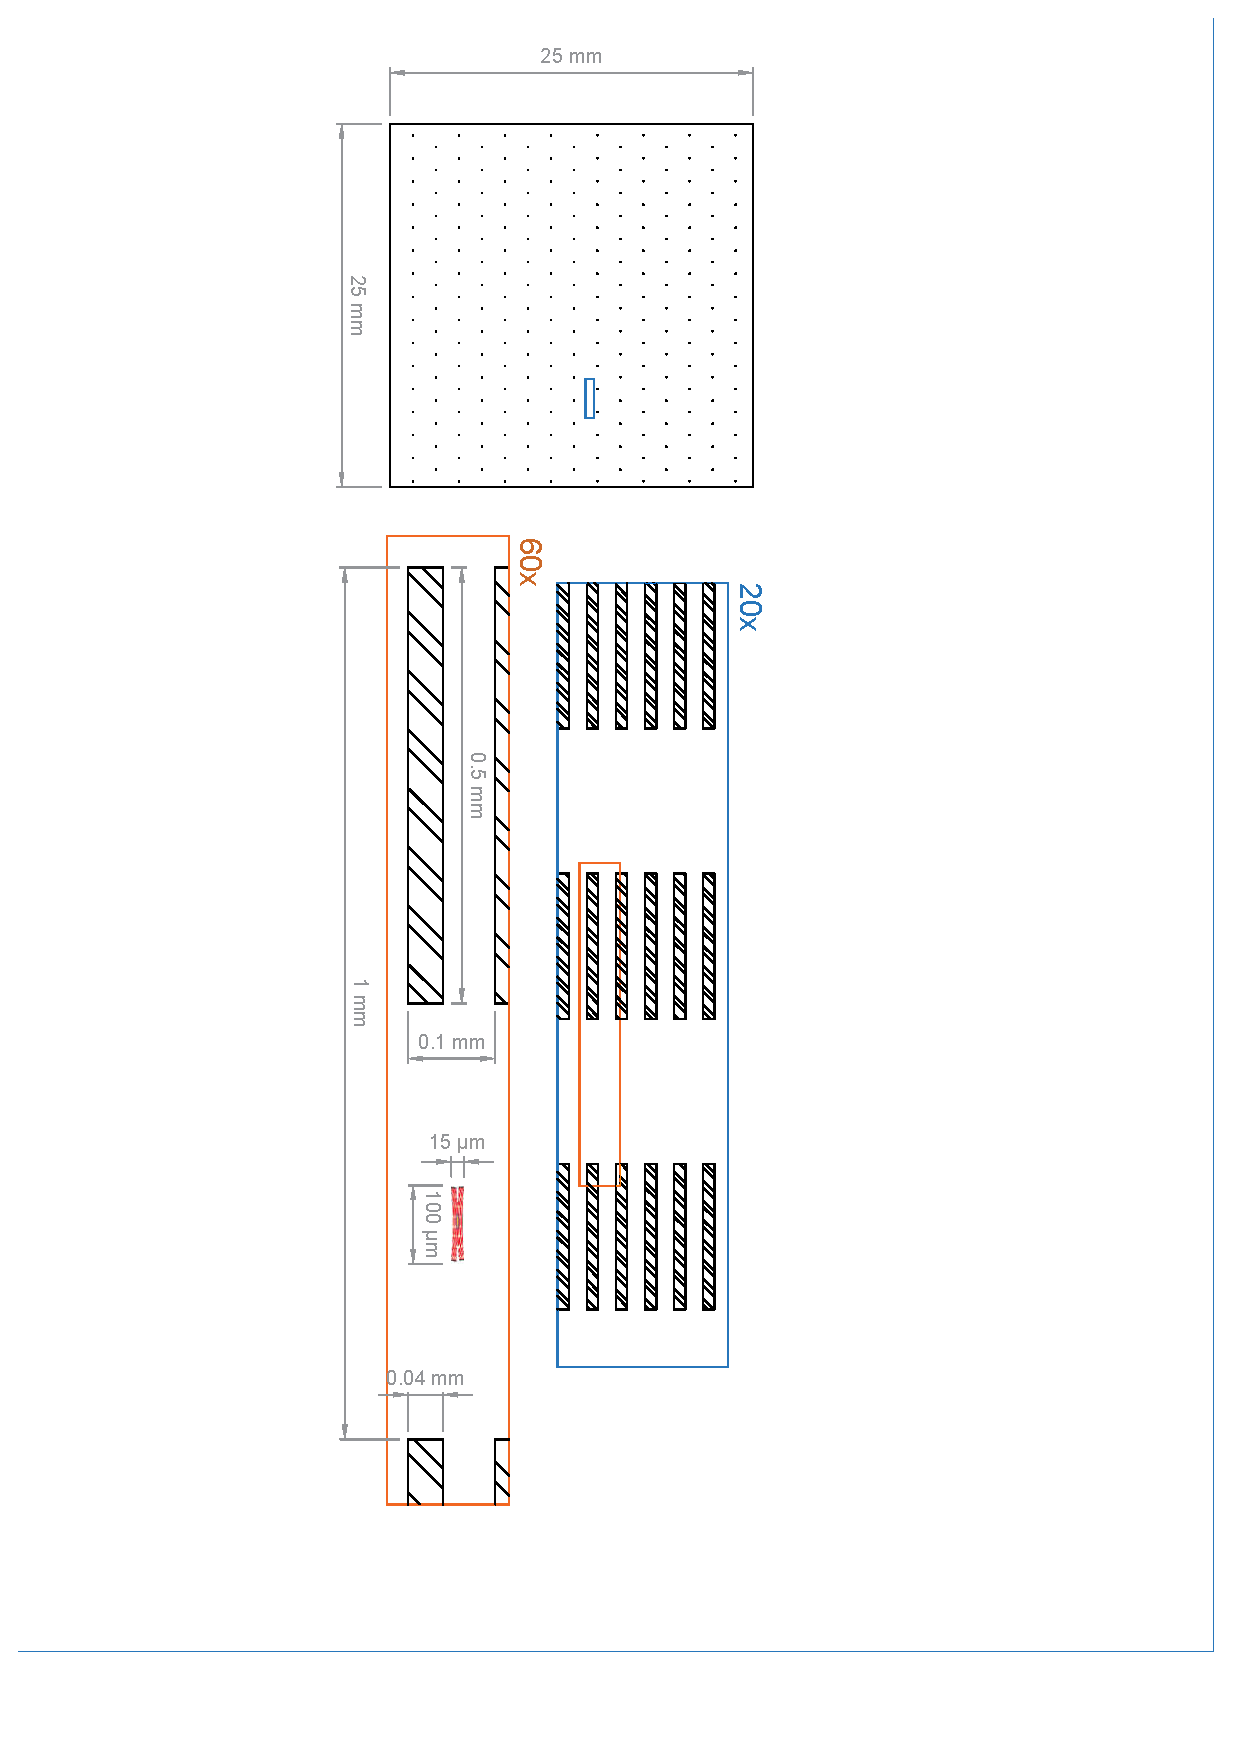
\includegraphics[trim={5cm 2cm 7cm 0.5cm}, clip, width = 5.4 cm, angle = 90]{fig/Verificacion_Teorema/geometry}
	\caption{geometry used to solve the exact problem. } \label{fig:geometry}
\end{figure}

A unstructured mesh composed by triangles of 0.1 [mm] characteristic size is used for the exact problem, which is refined near collagen inclusions in order to correctly consider the meso-scale into the model. Refined elements has a characteristic size of 0.0075 [mm]. On the other hand, the mesh used to solve the homogenized problem has a characteristic length of 0.1 [mm]. This difference is a consequence of the fact that homogenized model does not need explicitly the mesoscale in the mesh, because the mesoscopic properties are already considered in the effective macroscopic diffusion tensor. The mesh size for the homogenized problem is selected in order to have at least (usually more) one node per each inclusion, which is useful for randomly generated fibrotic meshes, that will be used in some experiments. For this case, a even more coarse mesh can be used, given the constant value of $\theta_c$ and $\theta_f$.

In order to quantify the approximation error at each time step, we can use the L2-norm, this is:

\begin{equation}
\text{error} = \frac{\norm{\phi - \phi_h}_{L2}}{\norm{\phi}_{L2}} = \frac{\int_{\Omega} (\phi - \phi_h)^2 d\Omega}{\int_{\Omega} \phi^2 d \Omega} \label{eq:errorL2}
\end{equation}

The final error obtained has three sources: the homogenization, the use of a coarse mesh in the homogenized problem, and the interpolation of the exact solution in the coarser mesh in order to calculate the error. Is mandatory to isolate the homogenization error from the mesh produced error. We did this by solving the equations over a tissue without collagen ($\theta = 0$). So, with this result, we chooses the mesh described above keeping the L2$-$error of the mesh coarseness below $10^{-2}$.

\begin{figure}[!htbp]
	\centering
	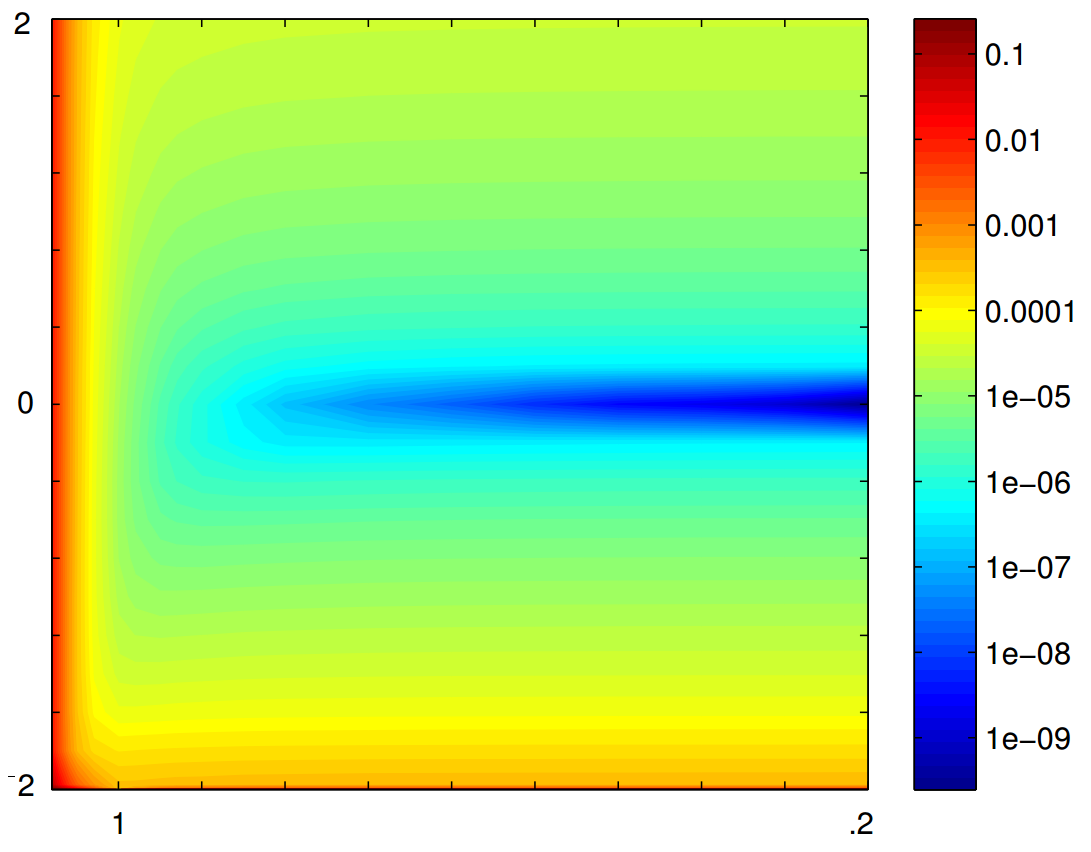
\includegraphics[height = 4.5 cm]{fig/Verificacion_Teorema/comparison_MEJORAR_SI_ALCANZO}
	\caption{Plot of L2-error for different mesh sizes and $\beta$ values (log scale on $\phi$). The horizontal axis has the mesh refinement in millimeters. The vertical axis has the $\beta$ values.} \label{fig:errorR1}
\end{figure}


In order to verify the established above, we  can solve the stationary version of \eqref{eq:diff_weak_form} for different mesh sizes and $\beta$ values, as can be seen in th Figure \ref{fig:errorR1}, where we can see that the homogenized solution converges to the exact one when $\beta \rightarrow 0$ and mesh size becomes equal to the mesh size for the exact problem.

\begin{figure}[!htb]
	\centering
	
\includegraphics[height = 3 cm, trim = {6cm 6cm 6cm 6cm}, clip]{fig/Verificacion_Teorema/20}
	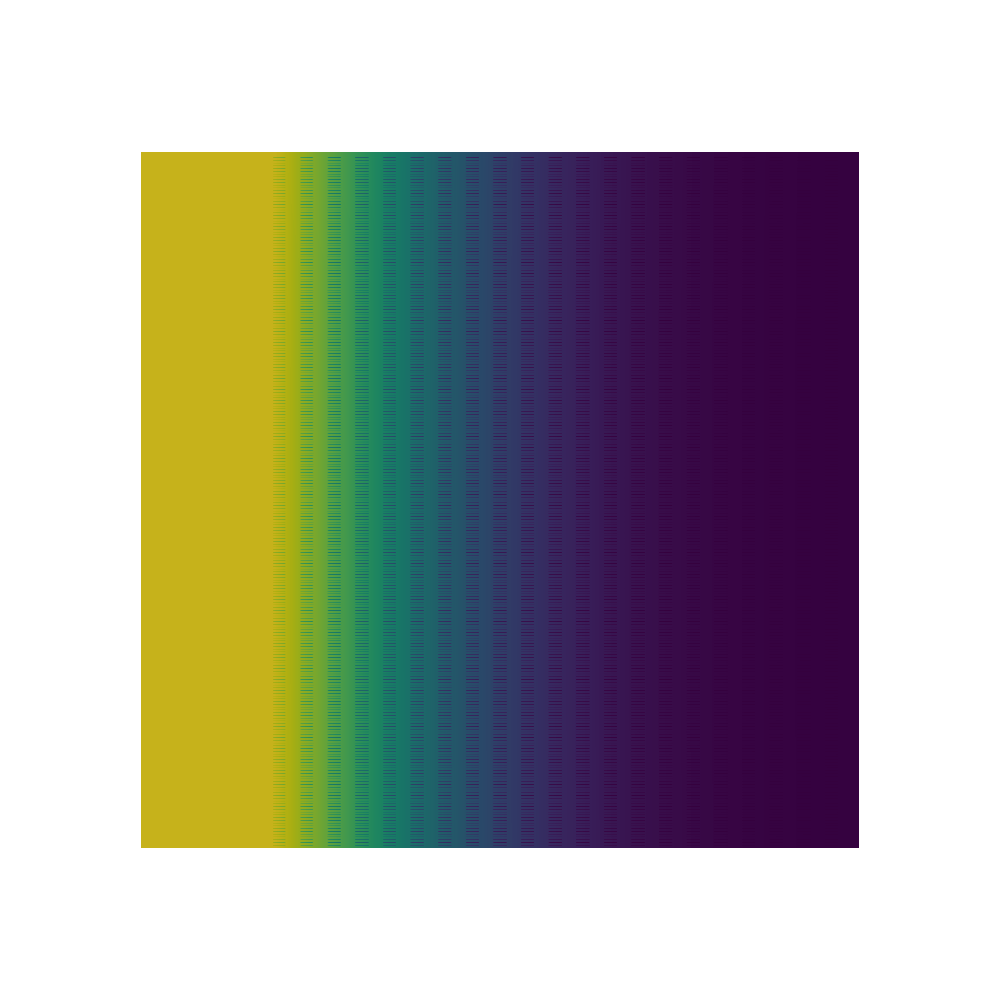
\includegraphics[height = 3 cm, trim = {6cm 6cm 6cm 6cm}, clip]{fig/Verificacion_Teorema/250}
	
\includegraphics[height = 3 cm, trim = {6cm 6cm 6cm 6cm}, clip]{fig/Verificacion_Teorema/500}
	
\includegraphics[height = 3 cm, trim = {6cm 6cm 6cm 6cm}, clip]{fig/Verificacion_Teorema/700}
	
\includegraphics[height = 3 cm, trim = {6cm 6cm 6cm 6cm}, clip]{fig/Verificacion_Teorema/20h}
	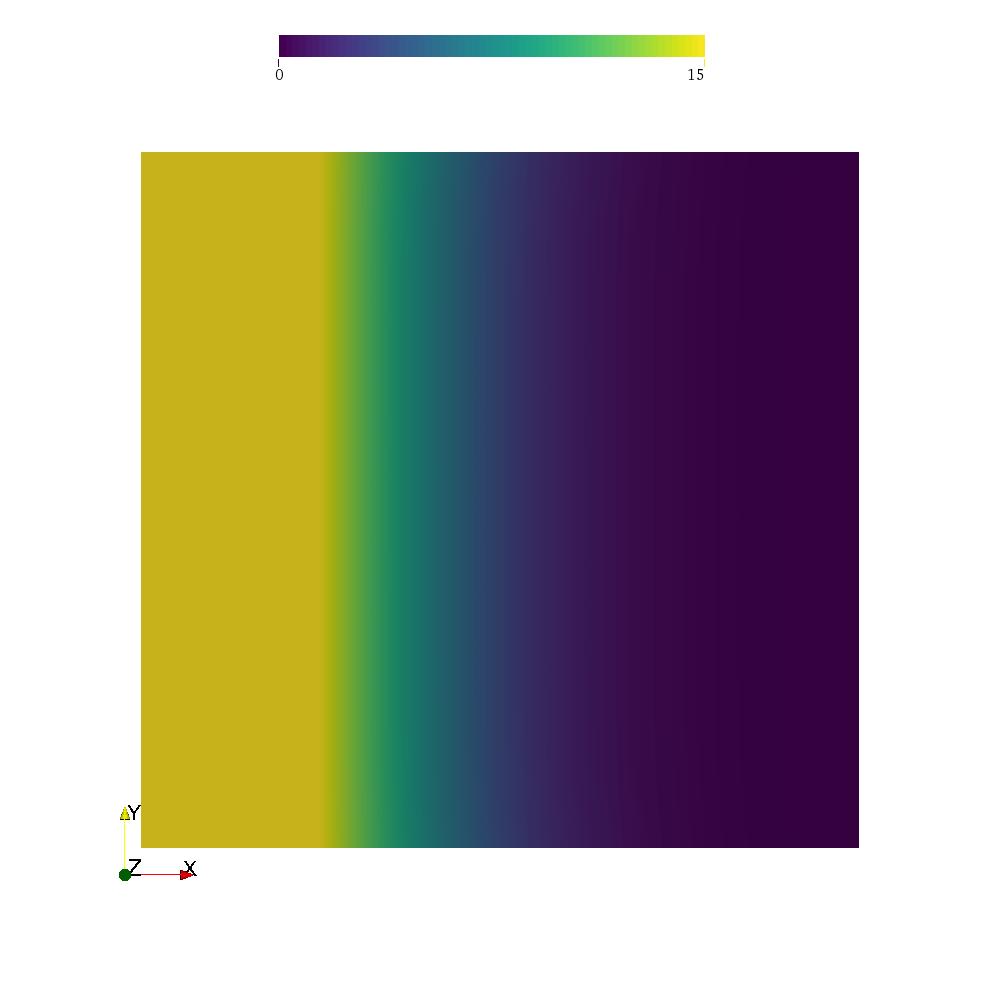
\includegraphics[height = 3 cm, trim = {6cm 6cm 6cm 6cm}, clip]{fig/Verificacion_Teorema/250h}
	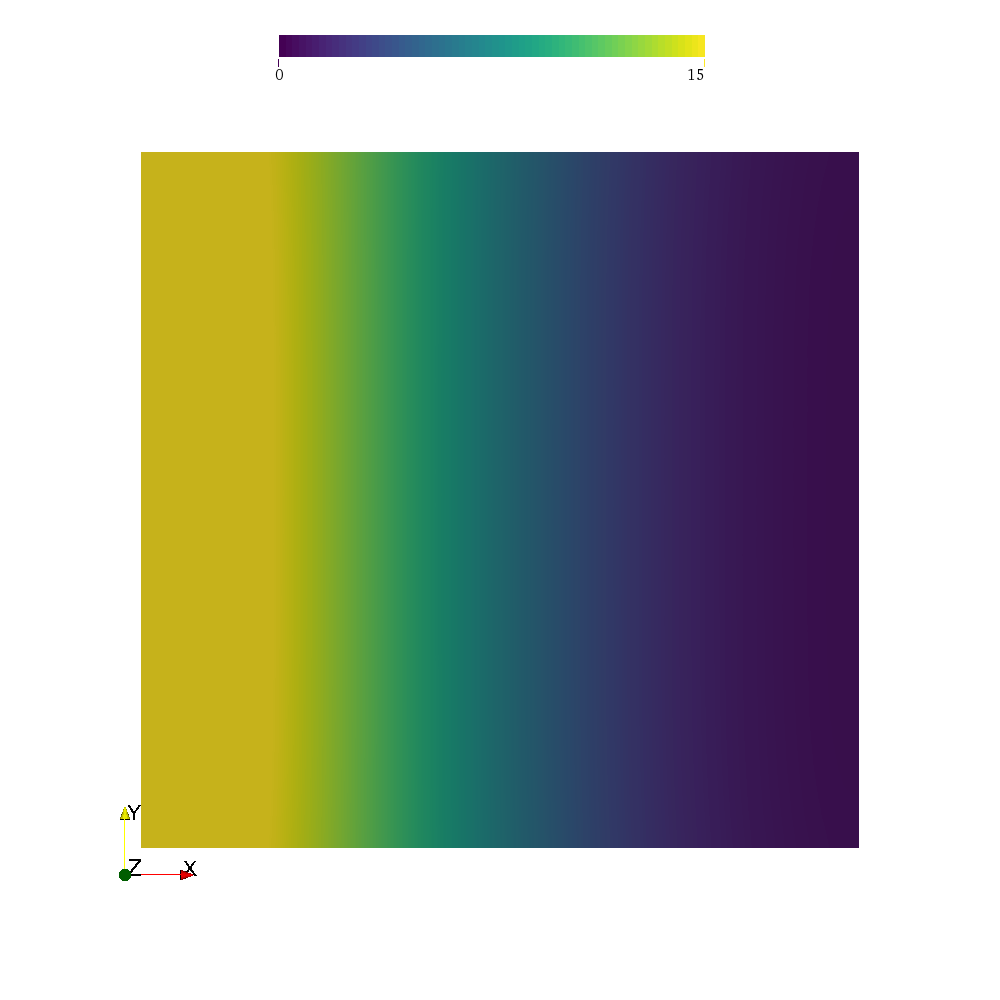
\includegraphics[height = 3 cm, trim = {6cm 6cm 6cm 6cm}, clip]{fig/Verificacion_Teorema/500h}
	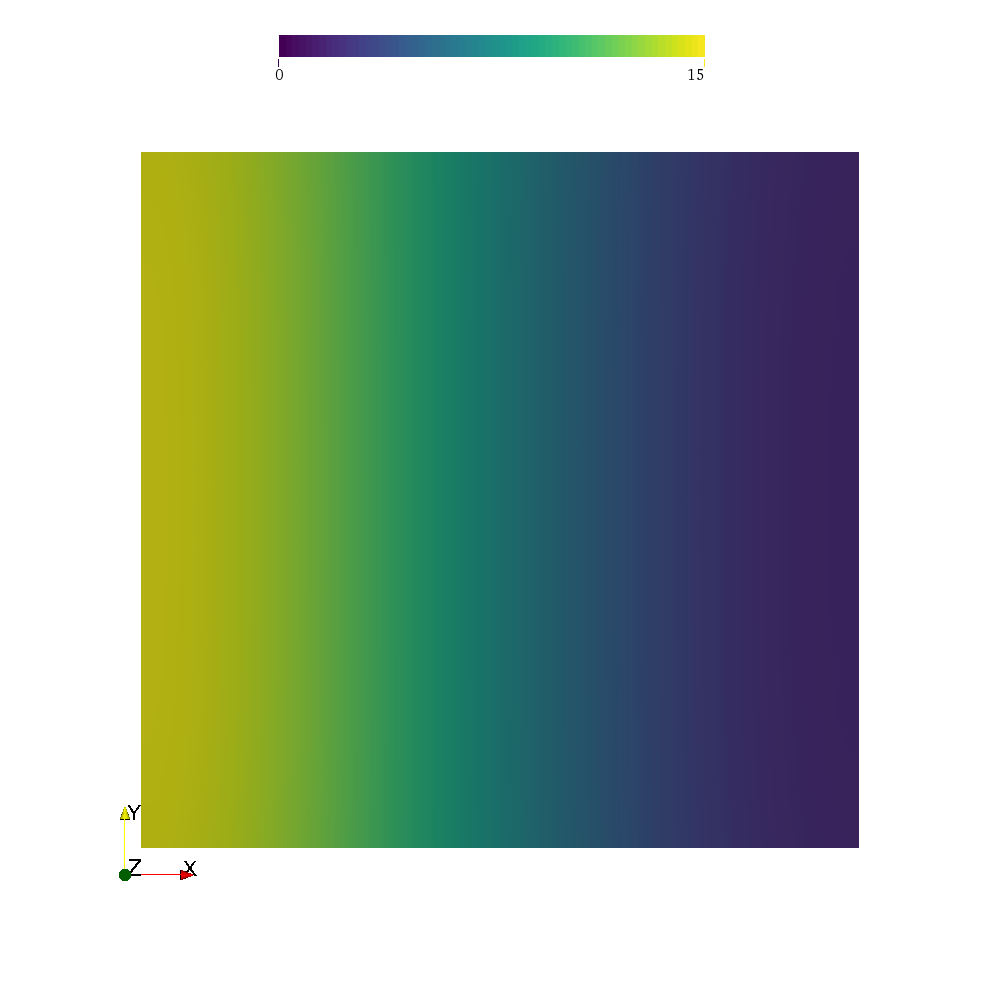
\includegraphics[height = 3 cm, trim = {6cm 6cm 6cm 6cm}, clip]{fig/Verificacion_Teorema/700h}\\[0.3 cm]
	
	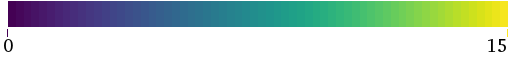
\includegraphics[height = 0.7 cm]{fig/Verificacion_Teorema/colourbar_diffusion}	
	\caption{Temporal evolution of the exact (up) and the homogenized (down) solution. From left to right we have $t = 20 ms$, $t = 250 ms$, $t = 500 ms$, $t = 700 ms$.} \label{fig:surrogate_ver}
\end{figure}

The evolution of both exact and homogenized solutions in time can be appreciated in figure \ref{fig:surrogate_ver}, and the error time evolution is in figure \ref{fig:verification_error_L2}. The error decrease in time, as is expected. Also, it can be noted that the error is greater when $\nabla \phi$ is greater, as is expected too, because the diffusion term is homogenized only. So, if diffusion decreases then L2$-$error also decreases.

This example is a worst-case-scenario, because the collagen inclusions are huge. In fact, from a physiological point of view, the values of $\theta_c$ and $\theta_f$ describes a very fibrotic tissue.


It has to be noted that the conduction velocity (CV) is a little bit underestimated in the homogenized model. This is due to the existence of paths without collagen in the mesh for exact problem, i.e., there are some ways where the potential propagates withouth any obstacles, and this is not considered by the effective tensor. Nevertheless, the difference is small, and the behavior of homogenized solution is well enough to reproduce the potential reaction-diffusion, as we will see in the section of numerical experiments.

The finite element method was implemented by using the FEniCS \cite{FENICS} open source library, which is composed of DOLFIN, FFC, UFL, FIAT and UFC. The mesh was generated using the open-source program GMSH \cite{GMSH}. Both, FEniCS and GMSH were interfaced with Python codes.


\begin{figure}[!htb]
	\centering
	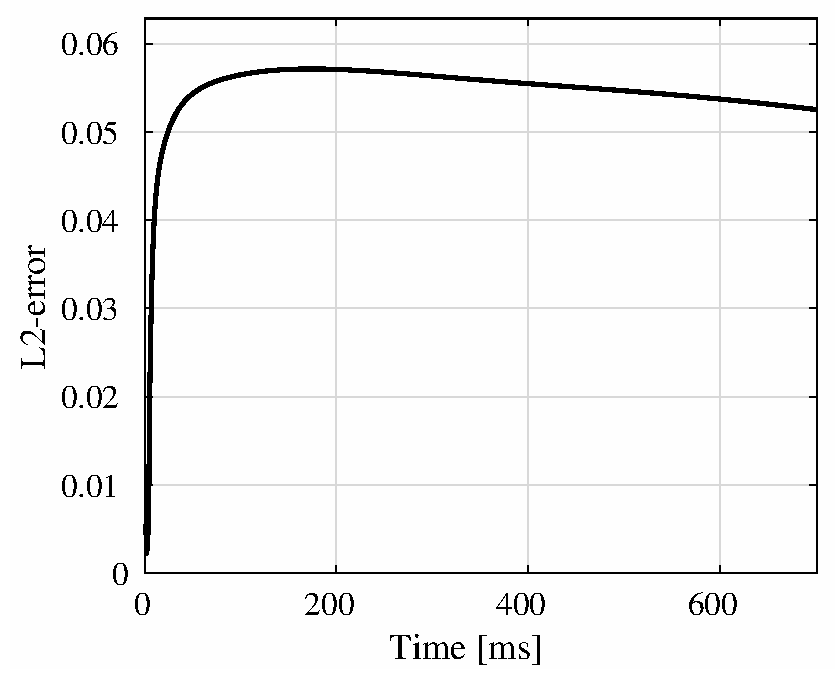
\includegraphics[height = 5 cm]{fig/Verificacion_Teorema/error_L2}
	\caption{Temporal evolution of L2-error for diffusion simulation.} \label{fig:verification_error_L2}
\end{figure}


\subsection{Discretization of the Minimal model}

The time discretization of the gating variables is semi-implicit. So first, for each time-step, the ODE's in \eqref{eq:mde_min} are solved using:


\begin{equation}
\arraycolsep=1.4pt\def\arraystretch{2.8}
\begin{array}{l}
r^{n+1} = \dfrac{r^n + (\Delta t r_{\infty}(1 - H(\phi - \theta_r)))/\tau_r^-}{1  +  (\Delta t (1 - H(\phi^n - \theta_r)))/\tau_r^- + (\Delta t H(\phi^n - \theta_r))/\tau_r^+} \\

w^{n+1} = \dfrac{w^n + (\Delta t w_{\infty}(1 - H(\phi - \theta_w)))/\tau_w^-}{1  +  (\Delta t (1 - H(\phi^n - \theta_w)))/\tau_w^- + (\Delta t H(\phi^n - \theta_w))/\tau_w^+} \\
   
s^{n+1} = \dfrac{s^n + \Delta t (1 + tanh(k_s (\phi^n - \phi_s)))/(2 \tau_s)}{(1 + \Delta t / \tau_s)}
\end{array}  \label{eq:mono_disc_gating}
\end{equation}

whose solutions are plugged in the PDE:

\begin{equation}
\dfrac{\phi^{n + 1} - \phi^n}{\Delta t}=  div(D \nabla \phi^{n+1}) - (J_{fi}^n + +  J_{si}^n + J_{so}^n) \label{eq:mono_disc_phi}
\end{equation}

The idea is to solve a stationary problem for each time step. This will be achieved trough a finite element method. 

Since we gonna use only Neumman boundary conditions for the numerical experiments, let us consider the test function space $V = \{ v \in H^1(\Omega) \}$. Multiplying \eqref{eq:mono_disc_phi} by a function of this space, integrating over all $\Omega$, considering the no-flux boundary conditions, and remembering the Green's Theorem, the weak form of the partial differential equation is obtained, so the problem can be re-written in the form $a (\phi^{n+1}, v) = L (v)$ as follows:

\begin{align}
a (\phi, v) = & \int_{\Omega} \phi v  d \Omega + \Delta t \int_{\Omega} D \nabla \phi \nabla v d \Omega \\
L (v) = & \int_{\Omega} \phi^n v d \Omega + \Delta t \int_{\Gamma_N} g v ds - \Delta t \int_{\Omega}( J_{fi}^n +  J_{si}^n + J_{so}^n )v d \Omega \label{eq:mde_min_weak}
\end{align}

where the notation $\phi = \phi^{n+1}$ is taken while there is no confusion in the meaning of the variables. Note that the currents are calculated using $\phi^n$, $r^{n+1}$, $w^{n+1}$ and $s^{n+1}$. 

Now, let us consider the finite dimensional space $V_h \subset V$ and the Galerkin method:

\begin{equation}
\phi = (c_1, c_2, ..., c_k) \cdot (\xi_1, \xi_2, ...., \xi_k) = \sum_{i=1}^k a_i \xi_i \label{eq:galerkin_method}
\end{equation}

where k is the total number of degrees of freedom, the functions $\{\xi_i \}_{i=1}^k$ belongs to the space $V_k$ and $c_i$ is the solution at the i-node. This way, the problem can be spatially discretized replacing \eqref{eq:galerkin_method} on equation \eqref{eq:mde_min_weak}. So, the problem is: find $\phi\in V$ such that $a_h (\phi, v) = L_h(v) \forall v\in V_h$, where 

\begin{align*}
a_h = & \int_{\Omega} (c_1, c_2, ..., c_k) (\xi_1, \xi_2, ...., \xi_k) \cdot (\xi_1, \xi_2, ...., \xi_k) ~ d \Omega \\
& + \Delta t \int_{\Omega} D (c_1, c_2, ..., c_k) (\nabla \xi_1, \nabla \xi_2, ...., \nabla \xi_k) \cdot (\nabla \xi_1, \nabla \xi_2, ...., \nabla \xi_k)~ d \Omega \\
L_h = & \int_{\Omega} (c_1^n, c_2^n, ..., c_k^n) (\xi_1, \xi_2, ...., \xi_k) \cdot (\xi_1, \xi_2, ...., \xi_k)~ d \Omega \\
& - \Delta t \int_{\Omega} (\gamma_1, \gamma_2, ..., \gamma_k) (\xi_1, \xi_2, ...., \xi_k) \cdot (\xi_1, \xi_2, ...., \xi_k)~ d \Omega
\end{align*}



where the test functions were discretized with $V_h$ functions. The current $J^n = J_{so}^n + J_{si}^n + J_{fi}^n$ was also discretized using $J = \sum_{i=1}^k \gamma_i \xi_i$. Now, defining the usually called \textsl{mass matrix}  $M \in \mathbb{M}_{k \times k}; M_{ij} = \int \xi_i \xi_j d \Omega $ and the \textsl{stifness matrix} $K \in \mathbb{M}_{k \times k}; K_{ij} = \int (D \nabla \xi_i) \cdot \nabla \xi_j d \Omega$, the discretized weak form yields to:

\begin{equation}
(M + \Delta t K) c^{n+1} = M c^n - \Delta t M \vec{\gamma} \label{eq:Ax=b}
\end{equation}

where $c^{n+1} = (c_1, c_2, ..., c_n)$ and $c^n = (c_1^n, c_2^n, ..., c_k^n)$. Finally, the space $V_h$ is chosen as the set of piecewise linear functions over each element.

The update of the \textsl{rhs} vector $(M c^n - \Delta t M \vec{\gamma})$ is done at each time-step, while the matrix $(M + \Delta t K)$ is just assembled once at the start of the simulation. Finally, we solve the linear system by using the conjugate gradient method. Also, in order to improve the convergence of the iterative method, an AMG preconditioner is applied before solving the linear system.


\subsection{Discretization of the FHN model}

The FitzHugh-Nagumo model can be plugged in the Monodomain equation \eqref{eq:MDE}, obtaining:  

\begin{equation}
\arraycolsep=2.5pt\def\arraystretch{2.8}
\begin{array}{rl}
\dfrac{\partial \phi}{ \partial t} = & div(D \nabla \phi) + c_1 \phi (\phi - \alpha)(1 - \phi) - c_2 w \\ 
\dfrac{\partial w}{\partial t} = & c_2 (\phi - wd)\\
\end{array}
 \label{eq:MONO+FHN}
\end{equation}

In order to better understand the numerical behavior of the problem, a stability analysis is performed in the following paragraphs.

\subsubsection{Stability Analysis}

The system \eqref{eq:MONO+FHN} is equivalent to:

\begin{equation} 
\phi \dfrac{\partial \phi}{ \partial t}  = \{ c_1 \phi (\phi - \alpha)(1 - \phi) - c_2 r \}\phi
\end{equation}

\begin{equation}
r \dfrac{\partial r}{\partial t}  = \{ c_2 (\phi - rd) \} r
\end{equation}

Now, adding both equations and defining E as:
\begin{equation}
\phi \dfrac{\partial \phi}{ \partial t} + r \dfrac{\partial r}{\partial t} = \frac{1}{2} \frac{d}{dt} \left(\phi^2 + r^2 \right):= E
\end{equation}

we obtain:

\begin{equation}
E = c_1 (1 + \alpha) \phi^3 - c_1 (\alpha \phi^2 +  \phi^4) -c_2 d r^2 \label{eq:total_energy}
\end{equation}

where the coupling term $c_2 \phi r$ has been canceledd. The E magnitude can be interpreted as the total energy of the system. In this context, results natural the anulation of the coupling term, since the energy cannot be generated in the ``interface'' of the system. Note that nearly all terms in the right side of equation (\ref{eq:total_energy}) dissipates energy from the system, in exception of $c_1 (1 + \alpha) \phi^3$, that constitutes a potential instability source. So, the balance between this last and the others terms conditions the decay of the solution.

Its desirable that the discretized version of the  system preserves the stability properties of the continuous system. To evaluate this, a general $\theta-$scheme can be used for the time discretization of the EDO, while a ``$\beta-$scheme'' can be used for the PDE, where the discretization has been done in order to obtain a linear problem:

\begin{equation}
\arraycolsep=1.4pt\def\arraystretch{2.2}
\begin{array}{rl}
\dfrac{r^{n+1}-r^n}{\Delta t} 
= &\{ \beta (c_2 \phi^{n + 1}) + (1 - \beta  )(c_2 \phi^{n + 1}) \} 
- \{ \theta  (c_2 d r^{n + 1}) + (1 - \theta )c_2 d r^{n} \} \\

\dfrac{\phi^{n+1} - \phi^n}{\Delta t}
= &c_1(1 + \alpha)\phi^n \{ \beta (\phi^{n+1})^2 + (1 - \beta) (\phi^{n})^2 \} 
- c_1 \alpha \{ \beta \phi^{n+1}  + (1 - \beta) \phi^n \} \\
&- c_1 (\phi^n)^2 \{ \beta \phi^{n+1} \} 
 - c_2 \{\theta r^{n+1} + (1 - \theta) r^{n} \}
\end{array} \label{eq:teta_esquema_MDE}
\end{equation}

where $\phi^{n}$ and $r^{n}$ are the potential and internal variable at the time step n, respectively. There exist, for instance, the following cases:

\begin{itemize}
\item $\theta = \beta = 0 \rightarrow$  explicit (forward Euler) and uncoupled problem.
\item $\theta = 1$ and $\beta = 1 \rightarrow$ implicit (backward Euler) and coupled problem.
\item $\theta = 1/2$ and $\beta = 1/2 \rightarrow$ implicit (Crank-Nicolson) and coupled problem.  
\end{itemize}

In general, for $\beta$ and $\theta$ greater than a half, implicit schemes will be obtained. To understand the energy change of the discrete system in time the equations (\ref{eq:teta_esquema_MDE}) are multiplied by $r^{n + \theta}$ and $\phi^{n + \beta}$ up and down, respectively, were the notation $a^{n + \theta} := \theta a^{n+1} + (1 - \theta), a^n$ has been adopted. Now, after some algebra arrangements the following is obtained:

\begin{equation}
\arraycolsep=1.4pt\def\arraystretch{2.2}
\begin{array}{llr}
\overline{E}:= & \dfrac{1}{2} \dfrac{r^{n+1}}{dt} - \dfrac{1}{2} \dfrac{r^{n}}{dt} + \dfrac{1}{2} \dfrac{\phi^{n+1}}{\Delta t} - \dfrac{1}{2} \dfrac{\phi^{n}}{\Delta t} \\

& = c_2 \phi^{n + \beta} r^{n + \theta} 
- c_2 d (r^{n + \theta})^2 
- \red{(\theta - \frac{1}{2}) \frac{1}{\Delta t} (r^{n+1} - r^n)^2} 
+ c_1 (1 + \alpha) \phi^n (\phi^{n + \beta})^2 \\
& - c_1 \alpha (\phi^{n + \beta})^{2}
- c_1 (\phi^n)^2 (\phi^{n + \beta})^2
- c_2 r^{n + \theta} v^{n + \beta}
- \red{(\beta - \frac{1}{2}) \frac{1}{\Delta t} (\phi^{n+1} - \phi^n)^2 }
\end{array}
\end{equation}

where $\overline{E}$ is the total ``\textsl{numerical energy}'' of the system. Note that the terms in red are not present in the continuos stability analisys, so is desirable, in order to preserve stability properties of the continuous system, that this term does not add energy to the system, is achieved simply by considering $\theta \geqslant 0.5$ and $\beta \geqslant 0.5$.

Finally, the following \textsl{semi-implicit} squeme is adopted:

\begin{equation}
\arraycolsep=1.4pt\def\arraystretch{2.2}
\begin{array}{llr}
\dfrac{r^{n+1} - r^n}{\Delta t} = c_2 \phi^n - c_2 d r^{n+1} \\
\dfrac{\phi^{n+1} - \phi^n}{\Delta t} = c_1 (1 + \alpha) (\phi^n)^2 - c_1 \alpha \phi^{n+1} - c_1 (\phi^n)^3 + div(D \nabla \phi^{n+1})
\end{array} \label{eq:FHN_semi_imp}
\end{equation}

where all the non-linear terms has been left explicit, and the linear ones has been left implicit. Also, the potential in the internal FHN equation has been left explicit, in order to finally obtain a linear and uncoupled problem. Note that the diffusion term has been added and was left implicit, in order to circunvent the well-knowed stability issues of a explicit diffusion term.

\subsubsection{Weak Form}

The weak variational form of the time-discretized PDE must to be written in order to perform a FEM discretization of the space. The variational form at each time step $n$ is $a(\phi^{n + 1}, v) = L(v)$ 

\begin{equation}
\arraycolsep=1.4pt\def\arraystretch{3}
\begin{array}{rcl}
a (\phi^{n + 1}, v)& = & \displaystyle \int_{\Omega} (1 + \Delta t c_1 \alpha) \phi^{n+1} v ~d \Omega + \Delta t \int_{\Omega} D \nabla \phi^{n+1} \nabla v ~d \Omega \\
L(v)& = &\displaystyle \int_{\Omega} \phi^n v ~d \Omega + \Delta t \int_\Omega \{ c_1(1 + \alpha)(\phi^n)^2 - c_1 (\phi^n)^3 - c_2 r^{n+1} \} v~ d \Omega + \Delta t \int_{\Gamma_N} g  v ~ds 
\end{array} \label{eq:esquema_definitivo}
\end{equation}


Now we can solve the problem by first solving the internal gatting variable equation and then solving \eqref{eq:esquema_definitivo}

\subsection{Experiment \# 1: Single Cell}

\subsubsection{Results Using FHN Reaction Model:}


First, a case with a small domain can be simulated, where the spatial dependence can be neglected (single cell). In figure \ref{fig:fhn_nofisiologico2} we can see the solution in time. As initial conditions we take $\phi(0) = 0.2 [mV]$ and $r(0) = 0$. The time step is $1 [ms]$. 

\begin{figure}[H]
\centering 
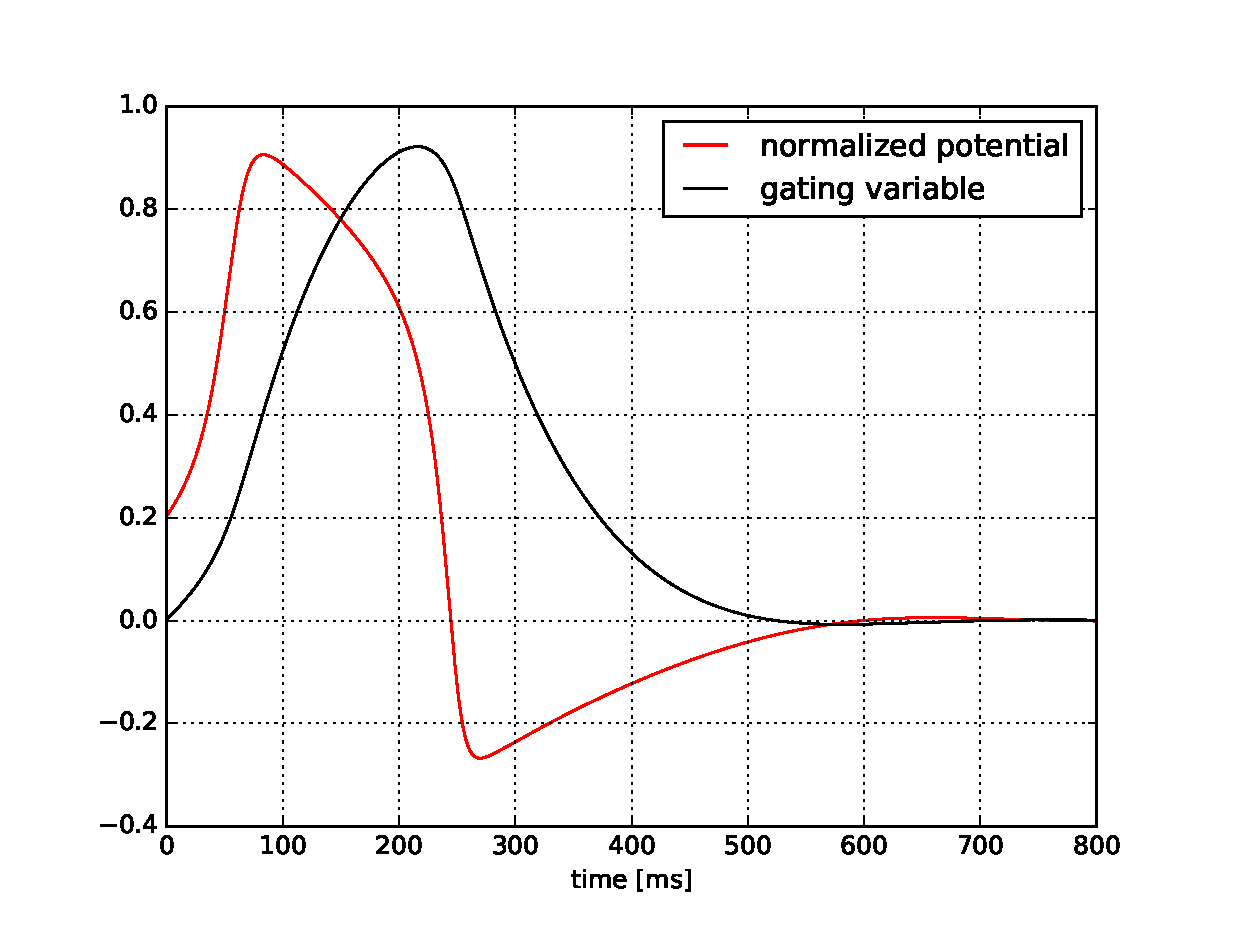
\includegraphics[height = 6 cm]{fig/Numerical_Experiments/ex1/EX1-FHN_single_cell.eps}
\caption{numerical solution of the FitzHugh-Namuno equations.}
\label{fig:fhn_nofisiologico2}
\end{figure}

The parameters used to generate the results can be appreciated in the table \ref{tab:parametros_FHN}.

\begin{table}[!htbp]
\centering
\caption{ Parameters used in the simulation.}
\label{tab:parametros_FHN}
\begin{tabular}{@{}cccc@{}}
\toprule
Parameter & Description                    & Value & Units  \\ \midrule
$c_1$     & Excitation rate constant       & 0.175 & $1/ms$ \\
$c_2$     & Excitation decay constant      & 0.03  & $1/ms$ \\
b         & Recovery rate constant         & 0.011 & $1/ms$ \\
d         & Recovery decay constant        & 0.55  & -      \\
$\alpha$  & Normalized threshold potential & 0.08  & -      \\ \bottomrule
\end{tabular}
\end{table}
Other approaches closer to the fully implicit discretization were tested, in order to see how far the time-step can be reduced. Nevertheless, the difference is negligible ($\approx 0.5 ~[ms]$), so the use of other schemes was discarded, because is preferable to have a positive definite system with a little bit lower time-step than a non positive definitive system with a negligible gain in the time step. On the other hand, with a fully implicit scheme it was noted that the time step can be severely increased (nearly 18 times the semi-implicit value), but this approach is also not considered because the system becomes highly computational expensive.

\subsubsection{Results Using Minimal Reaction Model:}

We solve the equations \eqref{eq:mono_disc_phi} and \eqref{eq:mono_disc_gating} over a small domain using the Minimal model for the reaction term. The dimensionless voltage variable is re-scaled to obtain values inside the physiological range by using the equation $\phi_{mV} = 85.7 \phi - 84$ or $\phi_{mV} = 85.7 \phi - 80.9$ if the tissue belongs to the atrial chamber. Initial scaled conditions are $\phi = 0$, $r = 1$, $w = 1$ and $s = 0$. A stimulus of $52 [mV]$ is applied for $0.2 [ms]$, in order to reproduce the $Na^+$ channels overture, i.e., the transition to phase 1. Note that this value is over the threshold needed to generate the cells action potential. A time-step of $0.1 [ms]$ is used. The result of the implementation can be seen in the figure \ref{fig:mde_min_ex1_single-cell}.

\begin{figure}[!htbp]
	\centering
	\subfigure[epicardial cell.]{
		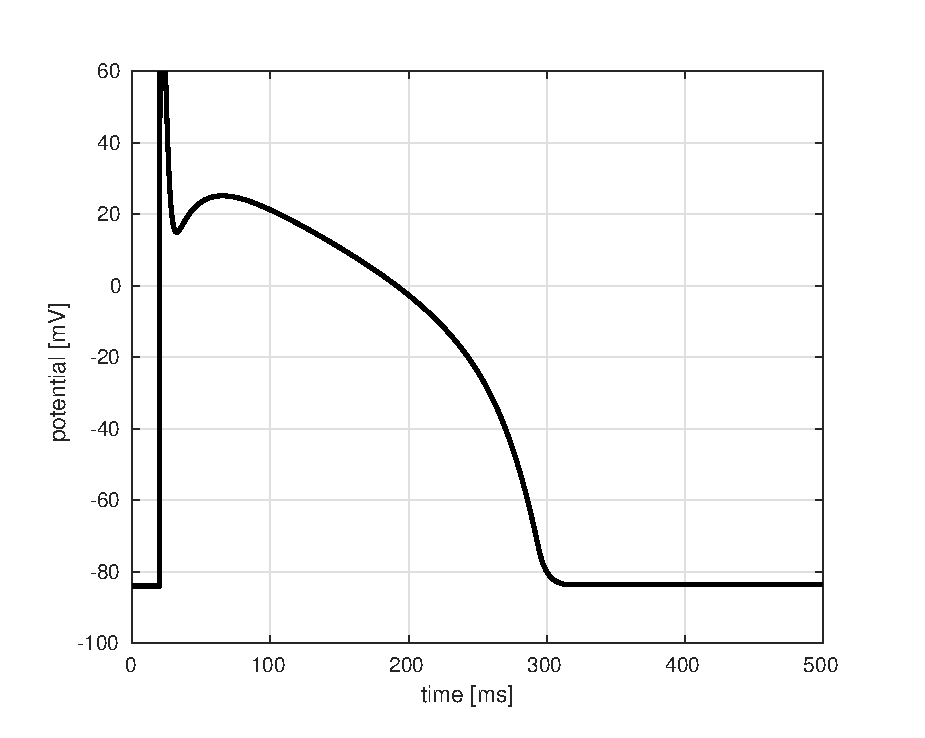
\includegraphics[width = 5 cm]{fig/Numerical_Experiments/ex1/ex1_min_epi}}
	\subfigure[endocardial cell.]{
		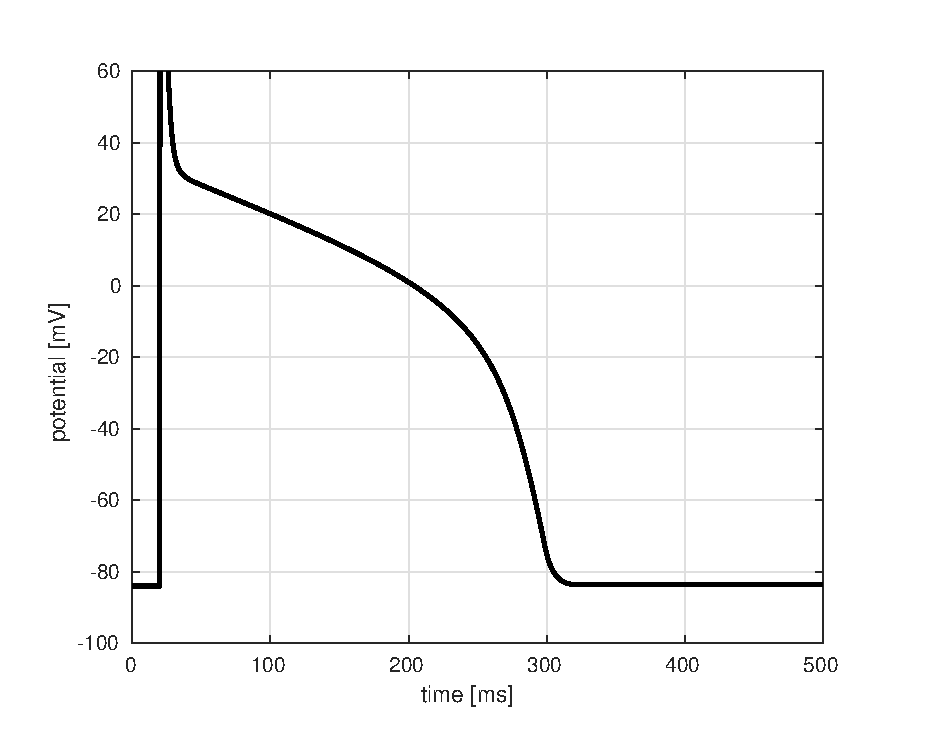
\includegraphics[width = 5 cm]{fig/Numerical_Experiments/ex1/ex1_min_endo}}
	\subfigure[mid-myocardial cell.]{
		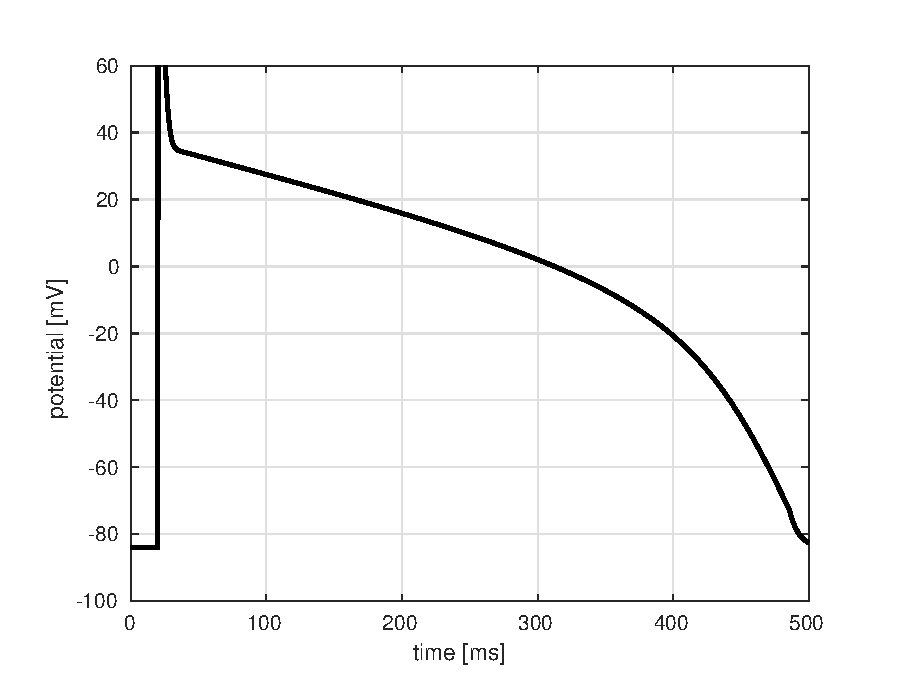
\includegraphics[width = 5 cm]{fig/Numerical_Experiments/ex1/ex1_min_mid}}
	\subfigure[atrial cell.]{
		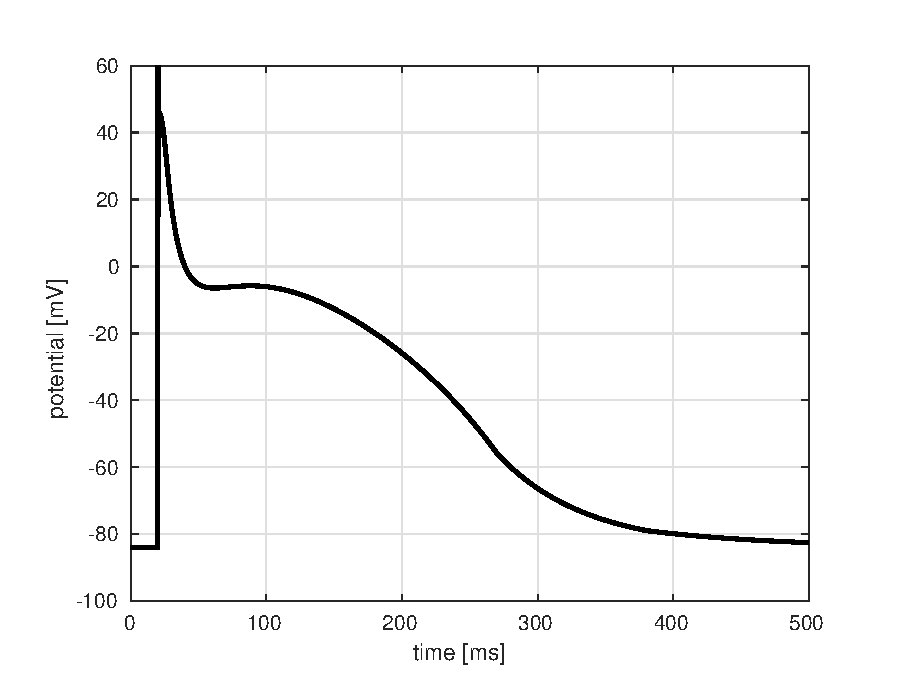
\includegraphics[width = 5 cm]{fig/Numerical_Experiments/ex1/ex1_min_atrial}}
	\caption{Simulated human AP for different configurations.} \label{fig:mde_min_ex1_single-cell}
\end{figure}	

If we look at the figures \ref{fig:fhn_nofisiologico2} and \ref{fig:mde_min_ex1_single-cell} we can observe the different advantages of the minimal model over the FHN: AP duration and shape are more realistic in the Minimal model and emulates better the refractory time, because by construction of the reaction model, the cell will can not repolarizate if is in phase 0, phase1, phase 2 or the beginning of phase 3. On the other hand, the FHN model is cheaper regards to computational cost but not enough to considerate FHN over Minimal. 

\subsection{Experiment \# 2: Tissue with High Fibrosis}

On this simulation we consider a cardiac tissue with high level of diffuse fibrosis. Both problems, exact and homogenized (surrogate model) will be compared. 

The geometry is a two dimensional $25 \times 25~mm^2$ square. A normalized stimulus of 1.587 for Minimal and 1.0 for FHN is applied in the left boundary during the first three seconds of the simulation. 

\subsubsection{Results Using FHN Cell Model:}

In the figure \ref{fig:ex2FHN} we can see the results of the simulations using the FHN reaction model, with the parameters of the table \ref{tab:parametros_FHN}. The potential is scaled to physiological range by using $\phi_{mv} = 110 \phi - 80$. The time step is $\Delta t = 0.5~[ms]$. The L2$-$error evolution with time is presented in figure \ref{fig:ex2_errorFHN}.

\begin{figure}[!htbp]
	\centering
	
\includegraphics[height = 3 cm, trim = {6cm 6cm 6cm 6cm}, clip]{fig/Numerical_Experiments/ex2/FHN/100}
	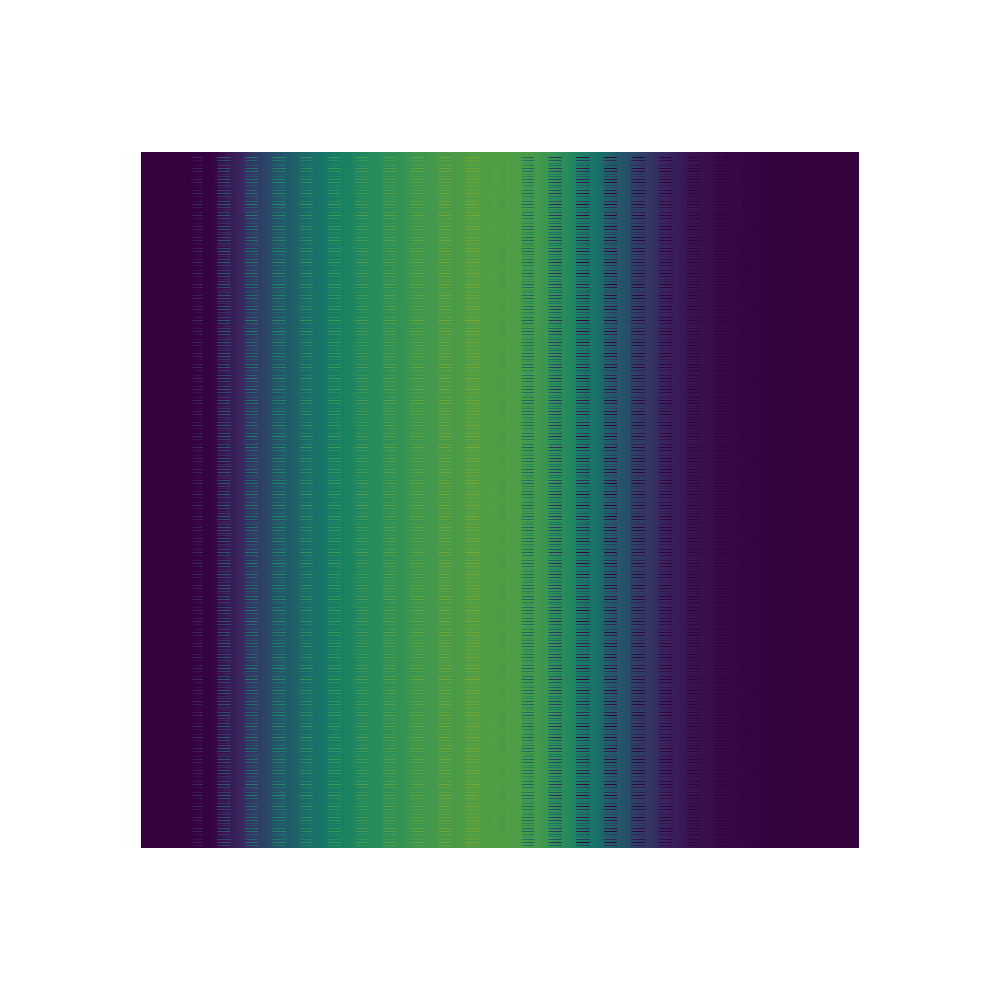
\includegraphics[height = 3 cm, trim = {6cm 6cm 6cm 6cm}, clip]{fig/Numerical_Experiments/ex2/FHN/250}
	
\includegraphics[height = 3 cm, trim = {6cm 6cm 6cm 6cm}, clip]{fig/Numerical_Experiments/ex2/FHN/390} \\
	
\includegraphics[height = 3 cm, trim = {6cm 6cm 6cm 6cm}, clip]{fig/Numerical_Experiments/ex2/FHN/100h}
	
\includegraphics[height = 3 cm, trim = {6cm 6cm 6cm 6cm}, clip]{fig/Numerical_Experiments/ex2/FHN/250h}
	
\includegraphics[height = 3 cm, trim = {6cm 6cm 6cm 6cm}, clip]{fig/Numerical_Experiments/ex2/FHN/390h} \\[0.3 cm]
	
	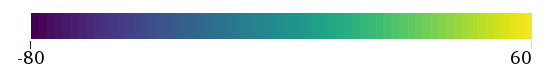
\includegraphics[height = 0.9 cm]{fig/Numerical_Experiments/colourbar_FHN}	
	\caption{temporal evolution of the exact (up) and the homogenized (down) solution. From left to right we have $t = 100 ms$, $t = 250 ms$ and $t = 390 ms$} \label{fig:ex2FHN}
\end{figure}

\begin{figure}[H]
\centering
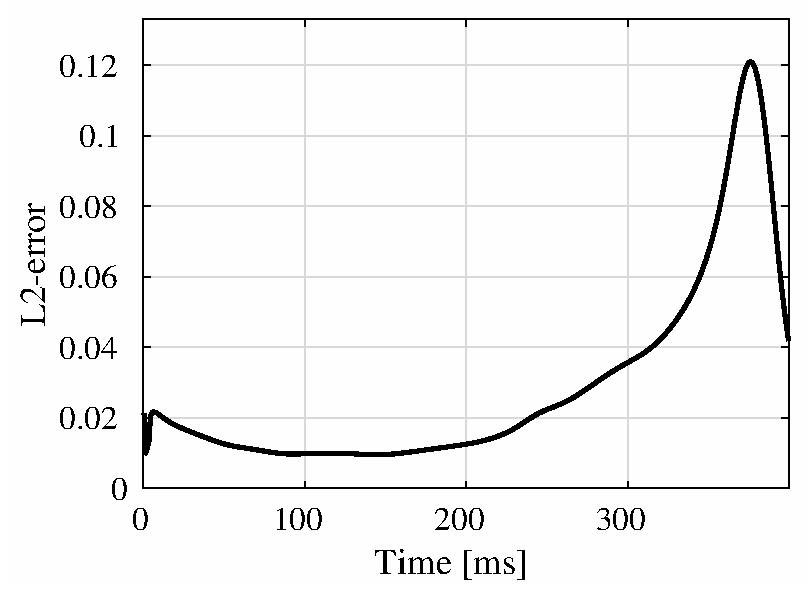
\includegraphics[height = 5 cm]{fig/Numerical_Experiments/ex2/FHN/error_L2}
\caption{L2-error evolution between exact and homogenized problem.} \label{fig:ex2_errorFHN}
\end{figure}

As can be appreciated, the surrogate models works good enough for the FHN reaction model from a macroscopic point of view.

\subsubsection{Results Using Minimal Gating Variables Model:}


In the figure \ref{fig:ex2Minimal} we can see the results of the simulations using the Minimal reaction model with atrial tissue parameters. The potential is scaled to physiological range by using $\phi_{mv} = 110 \phi - 80$. The time step is $\Delta t = 0.1~[ms]$. The results are presented in the figure \ref{fig:ex2Minimal}.

\begin{figure}[!htbp]
	\centering
	
\includegraphics[height = 3 cm, trim = {6cm 6cm 6cm 6cm}, clip]{fig/Numerical_Experiments/ex2/MINIMAL/3}
	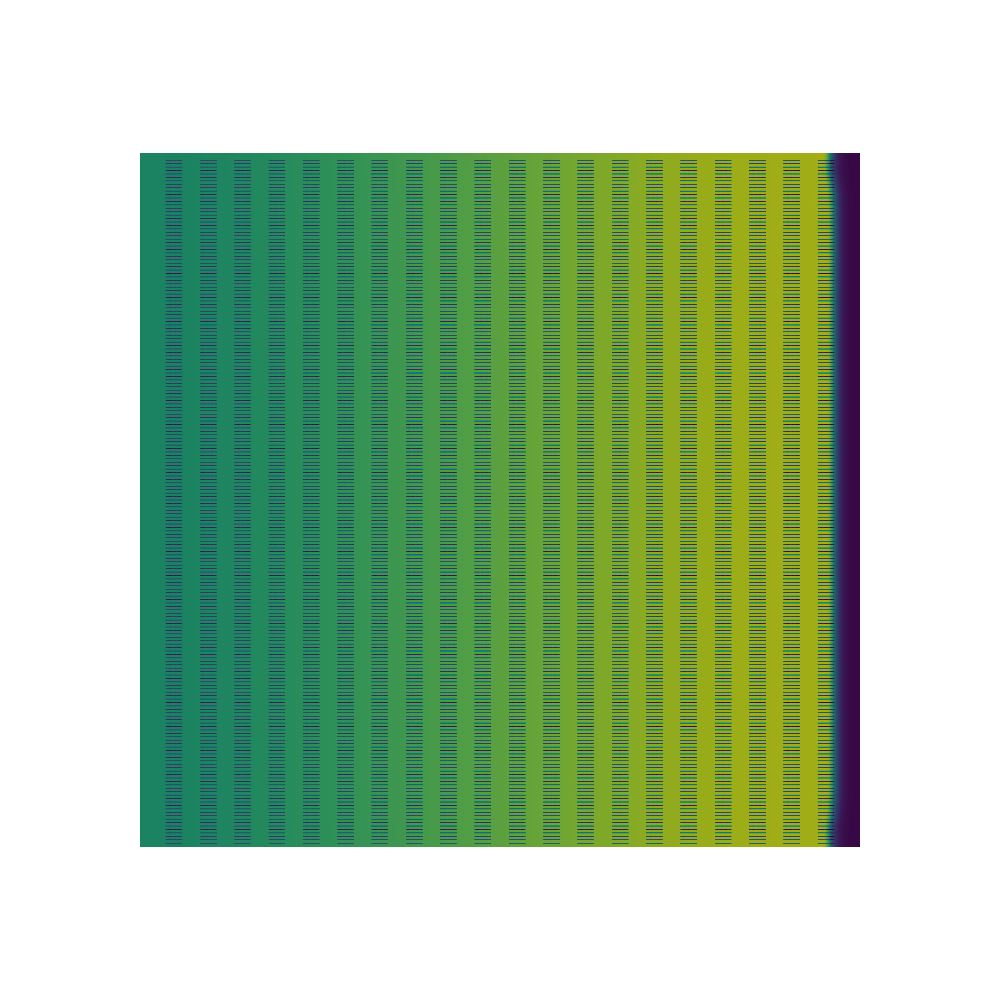
\includegraphics[height = 3 cm, trim = {6cm 6cm 6cm 6cm}, clip]{fig/Numerical_Experiments/ex2/MINIMAL/15}
	
\includegraphics[height = 3 cm, trim = {6cm 6cm 6cm 6cm}, clip]{fig/Numerical_Experiments/ex2/MINIMAL/30} \\
	
\includegraphics[height = 3 cm, trim = {6cm 6cm 6cm 6cm}, clip]{fig/Numerical_Experiments/ex2/MINIMAL/3h}
	
\includegraphics[height = 3 cm, trim = {6cm 6cm 6cm 6cm}, clip]{fig/Numerical_Experiments/ex2/MINIMAL/15h}
	
\includegraphics[height = 3 cm, trim = {6cm 6cm 6cm 6cm}, clip]{fig/Numerical_Experiments/ex2/MINIMAL/30h}  \\[0.3 cm]
	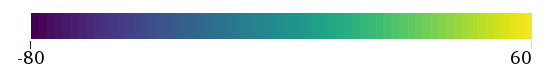
\includegraphics[height = 0.9 cm]{fig/Numerical_Experiments/colourbar_FHN}	
	\caption{Temporal evolution of the exact (up) and the homogenized (down) solution. From left to right we have $t = 3 ms$, $t = 250 ms$ and $t = 390 ms$} \label{fig:ex2Minimal}
\end{figure}


Note that the results are satisfactory, because the homogenized solution evolution reproduce the exact one in a mesoscopic scale, where interest of this study relays. The relative L2-error between both, the exact and homogenized solution, stay below totally acceptable values, as can be appreciated in figure \ref{fig:ex2_error}. 

\begin{figure}[!htbp]
	\centering
	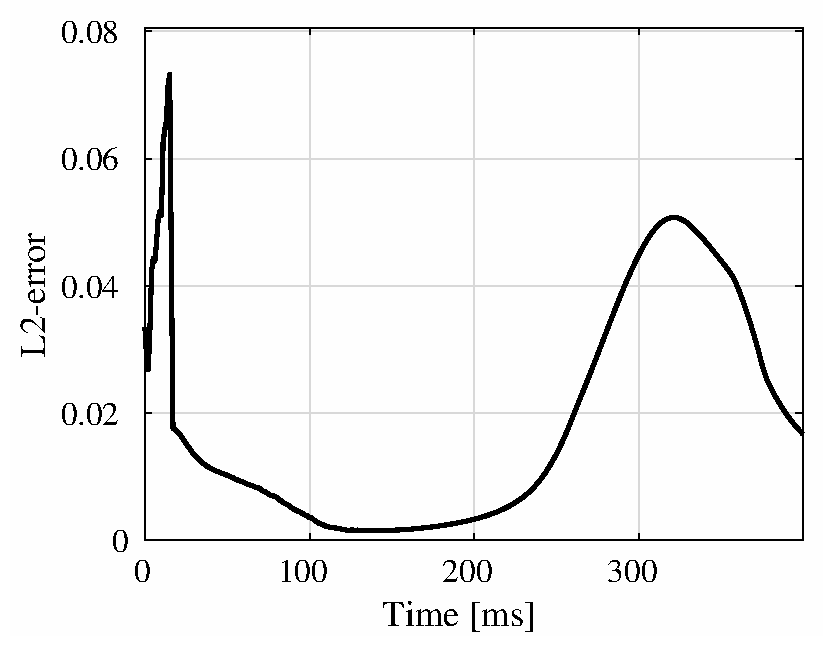
\includegraphics[height = 5 cm]{fig/Numerical_Experiments/ex2/MINIMAL/error_L2}
	\caption{L2-error evolution between exact and homogenized problem.} \label{fig:ex2_error}
\end{figure}

The first thing is to note how the front wave propagation is affected by the election of the reaction model. By inspection of the figures \ref{fig:ex2FHN} and \ref{fig:ex2Minimal} we can conclude that the front wave propagates faster in the minimal reaction model. Nevertheless, the mean behavior is quite similar in both FHN and Minimal models. A detailed view of the action potential for a cell located at the coordinates $(13~mm,~13~mm)$ is shown in the figure \ref{fig:cell_comparison}, where we can also note the difference between homogenized and exact problem. Furthermore, we can see how the surrogate model fits better with the exact solution when the Minimal reaction term is employed.

\begin{figure}[!htbp]
	\centering
	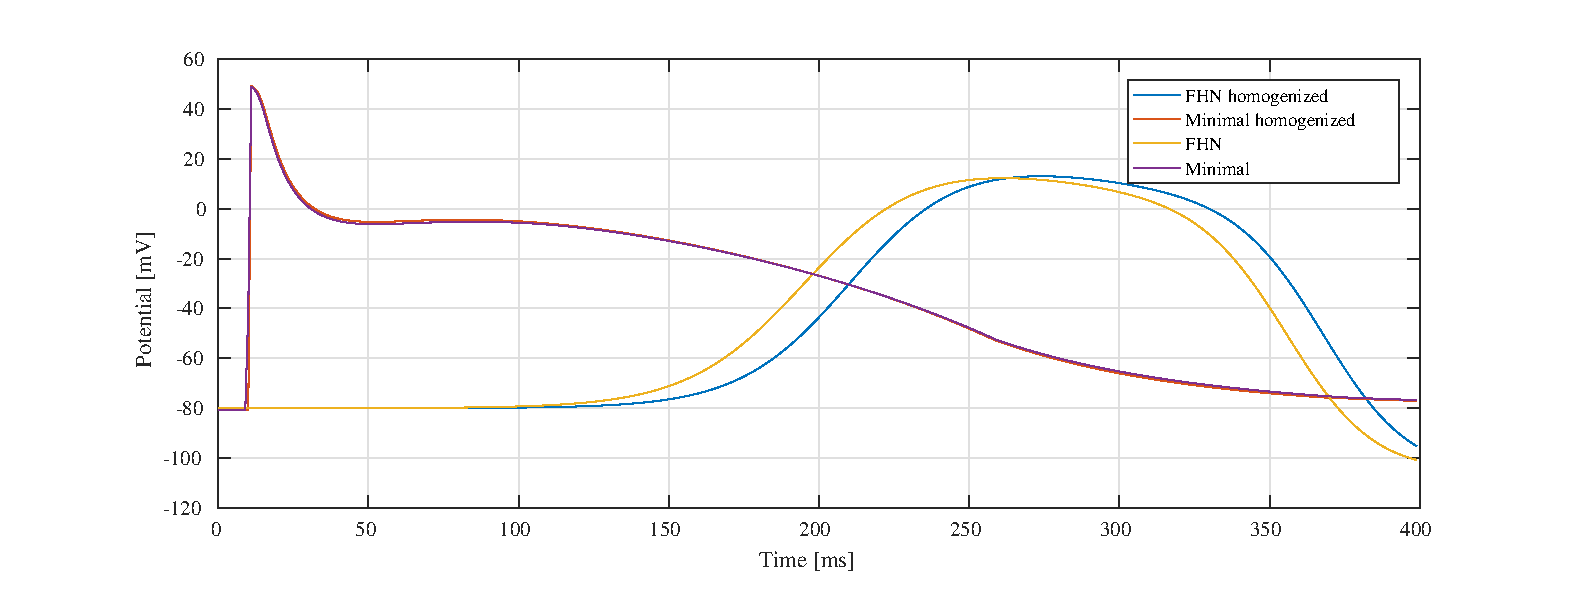
\includegraphics[height = 6.5 cm, trim ={2cm, 0cm, 0cm, 0cm}, clip]{fig/Numerical_Experiments/ex2/cell_comparison}
	\caption{Comparison of the action potential for a cell located at the coordinates $(13~mm,~13~mm).$}
	\label{fig:cell_comparison}
\end{figure}

\subsection{Experiment \# 3: Tissue with Stringy Fibrosis}

In this example the minimal model for mid-myocardial tissue will be used. Note that $\theta_c = 1$, so now there are vertical obstacles for the potential diffusion, as in figure \ref{fig:ex3_geo}. The reason to choose this configuration relays in impose a difficult case for the effective tensor. Characteristic mesh sizes are the same as previous examples.

\begin{figure}[!htbp]
\centering
\includegraphics[trim={4.1cm 2cm 6cm 0.5cm}, clip, width = 6cm, angle = 90]{fig/Numerical_Experiments/ex3/geometry}
\caption{Geometry for example \# 3.} \label{fig:ex3_geo}
\end{figure}

The stimulus is applied at the right edge for 3 milliseconds, and has a intensity of $52~[mV/mm]$. $\theta_f$ is 0.04 and the time step is 0.1 milliseconds. For the initial conditions we pick $\phi = 0$, $r = 1$, $w = 1$ and $s = 0$. The implementation results are presented in figure \ref{fig:results_exp3}.

\begin{figure}[!htbp]
\centering
\includegraphics[height = 0.8 cm]{fig/Numerical_Experiments/ex3/ex3_colourbar}\\[0.1 cm]
\includegraphics[height = 6 cm]{fig/Numerical_Experiments/ex3/results}
\caption{evolution of the potential over the tissue for the exact (up) and the homogenized (down) problem. From left to right, we have $t = 3~[ms]$, $t = 7~[ms]$ and $t = 15~[ms]$.} \label{fig:results_exp3}
\end{figure}

Note that homogenized solution reproduces the potential vertical blocking, which is natural considering the construction of the effective tensor. In summary, regards to the scale of study the result is satisfactory.

\subsection{Experiment \# 4: Tissue with Randomly Generated Fibrosis}

The collagen laminations are usually randomly distributed. In this example we try to emulate that by setting $\theta_c  \sim \mathcal{N}(\mu_c, \sigma_c)$ and $\theta_f \sim \mathcal{N}(\mu_f, \sigma_f)$, where $\sigma_c$ and $\mu_c$ are the mean and the standard deviation of a normal distribution. In particular, we will use the paramters of the table \ref{tab:ex4_parametros_random}:

\begin{figure}[!htbp]
	\centering
	\includegraphics[trim={7cm 3.5cm 5.5cm 3cm}, clip, width = 6cm, angle = 90]{fig/Numerical_Experiments/ex4/geometry}
	\caption{Geometry for example \# 4.} \label{fig:ex3_random}
\end{figure}

Note that the $\mathbb{E}(\theta_c)$ and $\mathbb{E}(\theta_f)$ represents a tissue with moderated level of fibrosis. In the figure \ref{fig:ex3_random} the geometry generated with the parameters of table \ref{tab:ex4_parametros_random} can be observed.

If the random values are not within a physiological range are then recalculated. For $\theta_c$ we admit values from 0.15 (healthy tissue) to 0.45 (highly fibrotic tissue), and for $\theta_f$ we admit values from 0.35 to 0.9. The choose of $\theta_f$ is done in order to get a tissue that emulates diffuse fibrosis, because values over 0.9 tends to generate collagen block-walls, i.e., stringy fibrosis. In addition, this example consider a stimulus with Gaussian distribution shape, with its maximum value located in the left-down corner. This allow us to see how the tissue anisotropy affects the wave propagation process, and how the surrogate model deals with it.

\begin{table}[!htbp]
	\centering
	\caption{Parameters used to generate random fibrotic tissue mesh.}
	\label{tab:ex4_parametros_random}
	\begin{tabular}{@{}cc@{}}
		\toprule
		Parameter  & Value \\ \midrule
		$\mu_c$    & 0.3   \\
		$\mu_f$    & 0.5   \\
		$\sigma_c$ & 0.2   \\
		$\sigma_f$ & 0.3   \\ \bottomrule
	\end{tabular}
\end{table}

\subsubsection{Results Using FHN Reaction Model}


The results and error evolution are shown in the figure \ref{fig:ex4FHN} and \ref{fig:ex4MIN_error_L2}, respectively. 

\begin{figure}[!htbp]
	\centering
	\includegraphics[height = 3 cm, trim = {6cm 6cm 6cm 6cm}, clip]{fig/Numerical_Experiments/ex4/FHN/100}
	\includegraphics[height = 3 cm, trim = {6cm 6cm 6cm 6cm}, clip]{fig/Numerical_Experiments/ex4/FHN/300}
	\includegraphics[height = 3 cm, trim = {6cm 6cm 6cm 6cm}, clip]{fig/Numerical_Experiments/ex4/FHN/500}
	\includegraphics[height = 3 cm, trim = {6cm 6cm 6cm 6cm}, clip]{fig/Numerical_Experiments/ex4/FHN/600} \\[0.1 cm]
	\includegraphics[height = 3 cm, trim = {6cm 6cm 6cm 6cm}, clip]{fig/Numerical_Experiments/ex4/FHN/100h}
	\includegraphics[height = 3 cm, trim = {6cm 6cm 6cm 6cm}, clip]{fig/Numerical_Experiments/ex4/FHN/300h}
	\includegraphics[height = 3 cm, trim = {6cm 6cm 6cm 6cm}, clip]{fig/Numerical_Experiments/ex4/FHN/500h}
	\includegraphics[height = 3 cm, trim = {6cm 6cm 6cm 6cm}, clip]{fig/Numerical_Experiments/ex4/FHN/600h}  \\[0.3 cm]
	\includegraphics[height = 0.9 cm]{fig/Numerical_Experiments/colourbar_FHN}	
	\caption{Temporal evolution of the exact (up) and the homogenized (down) solution. From left to right we have $t = 100 ms$, $t = 300 ms$,  $t = 500 ms$ and $t = 600 ms$} \label{fig:ex4FHN}
\end{figure}



\begin{figure}[!htbp]
	\centering
	\includegraphics[height = 5 cm]{fig/Numerical_Experiments/ex4/FHN/error_L2.eps}
	\caption{Temporal evolution of the error.}
	\label{fig:ex4MIN_error_L2}
\end{figure}


\subsubsection{Results Using Minimal Reaction Model}

The results for an Atrial tissue are shown in the figure \ref{fig:ex4Min} and the error is in figure \ref{fig:ex4_error_L2}. We can see an increase in the L2-error respect to the non-random case, which is a consequence of the experiment configuration. Notice that the wave propagation in the surrogate model fits better with the exact solution across the fiber direction than in the cross-fiber direction. This difference can be explained by considering the tissue anisotropy and the material proportions. In the fiber direction the collagen proportion at the meso-scale is smaller than in the vertical direction, therefore a better fit with the surrogate model in the fiber direction is expected.


\begin{figure}[!htbp]
	\centering
	\includegraphics[height = 3 cm, trim = {6cm 6cm 6cm 6cm}, clip]{fig/Numerical_Experiments/ex4/MINIMAL/3}
	\includegraphics[height = 3 cm, trim = {6cm 6cm 6cm 6cm}, clip]{fig/Numerical_Experiments/ex4/MINIMAL/10}
	\includegraphics[height = 3 cm, trim = {6cm 6cm 6cm 6cm}, clip]{fig/Numerical_Experiments/ex4/MINIMAL/20}
	\includegraphics[height = 3 cm, trim = {6cm 6cm 6cm 6cm}, clip]{fig/Numerical_Experiments/ex4/MINIMAL/35} \\[0.1 cm]
	\includegraphics[height = 3 cm, trim = {6cm 6cm 6cm 6cm}, clip]{fig/Numerical_Experiments/ex4/MINIMAL/3h}
	\includegraphics[height = 3 cm, trim = {6cm 6cm 6cm 6cm}, clip]{fig/Numerical_Experiments/ex4/MINIMAL/10h}
	\includegraphics[height = 3 cm, trim = {6cm 6cm 6cm 6cm}, clip]{fig/Numerical_Experiments/ex4/MINIMAL/20h}
	\includegraphics[height = 3 cm, trim = {6cm 6cm 6cm 6cm}, clip]{fig/Numerical_Experiments/ex4/MINIMAL/35h}  \\[0.3 cm]
	\includegraphics[height = 0.9 cm]{fig/Numerical_Experiments/colourbar_MINIMAL}	
	\caption{Temporal evolution of the exact (up) and the homogenized (down) solution. From left to right we have $t = 3 ms$, $t = 10 ms$,  $t = 20 ms$ and $t = 35 ms$} \label{fig:ex4Min}
\end{figure}


\begin{figure}[!htbp]
\centering
\includegraphics[height = 5 cm]{fig/Numerical_Experiments/ex4/MINIMAL/error_L2.eps}
\caption{Temporal evolution of the error.}
\label{fig:ex4_error_L2}
\end{figure}



\section{Conclusion and Perspectives}

We successfully obtained a model for the electric potential propagation in cardiac human tissue based on a classical reaction-diffusion approach using both FitzHugh-Nagumo and Minimal reaction terms. For future research, in order to get realistic enough simulations for the membrane cell activity regards to AP duration, AP shape and refractory time properties  we will consider the Minimal model only. Also, we can couple the Monodomain equations with a mechanical model for the cardiac tissue, since myocites has very elastic properties that affects the potential propagation.

The homogenization theory gives a very useful and effective tool to deal with fibered materials. By using some results of this theory, we obtained a surrogate model that severely improve the computational performance of the simulations, preserving the meso-scale properties in a mesh that only consider the macro-scopic scale. This surrogate model works fine for different configurations of fibrosis types, such as diffuse fibrosis and stringy fibrosis.

For future work, it will be necessary to apply the homogenization results in a three dimensional realistic geometry, considering the spatial variation of the lamination direction. Also, in order to evaluate the behavior of surrogate model in arrhythmia situations as a consequence of fibrosis, we have to study the spiral wave generation and break-up in cardiac tissue and see how the homogenized problem reproduces it.

Once we have all the above, one can go further and develop the inverse version of the electro-physiology problem, then use real electric potential measures to asses the fibrosis architecture and level of real patients, achieving finally a non-invasive way to diagnose pathological fibrosis.

As a final remark, it has to be noted that on this text we developed a tool for any kind of fibered material. Therefore, we can go beyond our bio-medical example and look for new applications of the surrogate model, wherever those materials arises.

\bibliographystyle{plain}
\bibliography{biblio_fibrosis}


\end{document}
\grid